\documentclass[bsc,frontabs,twoside,singlespacing,parskip]{infthesis}

\usepackage[textsize=small]{todonotes}
\usepackage{graphicx}
\usepackage[pagebackref]{hyperref}
\usepackage{subcaption}
\usepackage{algpseudocode}
\usepackage{algorithm}
\usepackage{url}
\usepackage{booktabs}
\usepackage{multirow}
\usepackage{amsmath}
\graphicspath{ {/afs/inf.ed.ac.uk/user/s09/s0954584/Dropbox/4th/unshredder/writing/imgs/} }
\setlength{\marginparwidth}{2cm}

\renewcommand*{\backref}[1]{}
\renewcommand*{\backrefalt}[4]{%
    \ifcase #1 (Not cited.)%
    \or        (Cited on page~#2.)%
    \else      (Cited on pages~#2.)%
    \fi}

\begin{document}

%\iffalse 
\title{Reconstructing Shredded Documents}
\author{Razvan Ranca}
\course{Artificial Intelligence and Computer Science}
\project{4th Year Project Report}
\date{\today}

\abstract{This project looks at the challenges involved in the automatic reconstruction of strip (vertically cut) and cross (both vertically and horizontally cut) shredded documents. The unshredding problem is of interest in the fields of forensics, investigative sciences, and archaeology. \vspace{1em}

All stages of the unshredding pipeline are analysed, starting from scanned images of shreds and ending with reconstructed documents. The current bottlenecks in this pipeline are identified and solutions are proposed. \vspace{1em}

The original contributions of this project include a probabilistic scoring function which outperforms the standard cost functions used in literature, a refinement upon a previously proposed, graph-inspired, search heuristic and a tractable up/down orientation method for strip-cut shreds.}

\maketitle
%\fi

\iffalse 
\begin{titlepage}
\begin{center}

\textsc{\LARGE \bf Reconstructing Shredded Documents} \vspace{2em}

\textsc{\Large Final year project} 

\vfill

\begin{minipage}{0.8\textwidth}
\centerline{\LARGE Abstract} \vspace{1em}

This project looks at the challenges involved in the automatic reconstruction of strip (vertically cut) and cross (both vertically and horizontally cut) shredded documents. The unshredding problem is of interest in the fields of forensics, investigative sciences, and archaeology. \vspace{1em}

All stages of the unshredding pipeline are analysed, starting from scanned images of shreds and ending with reconstructed documents. The current bottlenecks in this pipeline are identified and solutions are proposed. \vspace{1em}

The original contributions of this project include a probabilistic scoring function which outperforms the standard cost functions used in literature, a refinement upon a previously proposed, graph-inspired, search heuristic and a tractable up/down orientation method for strip-cut shreds.

\vspace{2em}
{\bf Keywords:} unshred; deshred; document reconstruction; shredder
\end{minipage} \vspace{10em}



\end{center}
\end{titlepage}
\fi


%\section*{Acknowledgements}
%Acknowledgements go here. 

\tableofcontents

%\pagenumbering{arabic}

\chapter{Introduction}
\label{chap1}
Ever since the paper shredder was invented, people have worked on sticking the pieces back together again. Recently, techniques permitting the purely electronic storage and transmittal of sensitive documents have been developed but, because of convenience or for legal reasons, many sensitive documents are still printed and eventually shredded. Traditionally, the cost of reconstructing these documents was considered prohibitive as the work had to be done manually (see Figure \ref{fig:iranDoc}), however with the development of methods that partly automate the process this situation is changing. 

It is currently unclear what level of security the paper shredder still offers.

\begin{figure}[h]
    \centering
    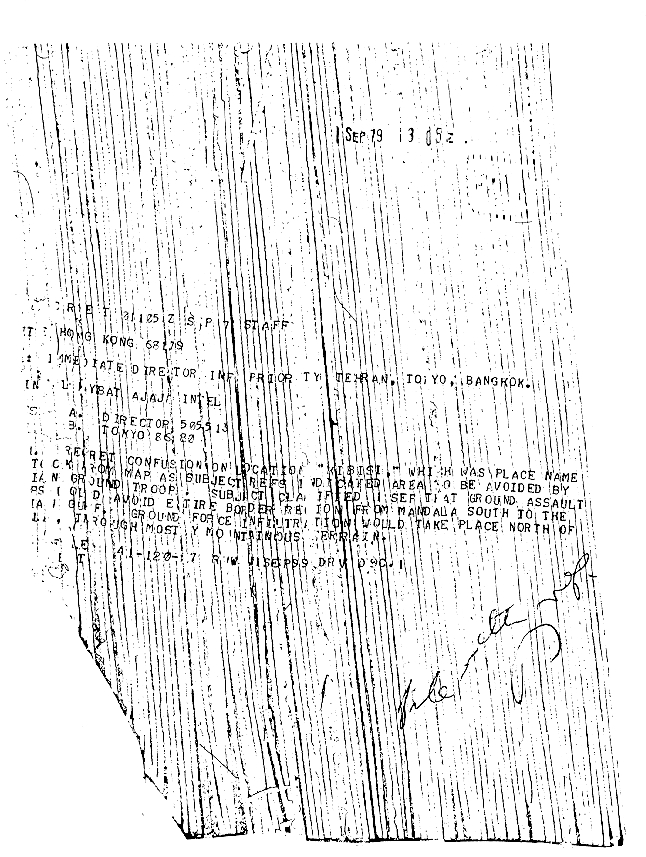
\includegraphics[width=0.5\textwidth, height=9cm]{iran}
    \caption{A shredded document belonging to the CIA. This was reconstructed by a team of carpet weavers during the 1979 Iran hostage crisis. The reconstructed documents were eventually released by the Iranian government in a series of books \cite{P10}}
    \label{fig:iranDoc}
\end{figure}

\section{Importance}
Techniques such as dumpster diving have long been used to gain access to sensitive information. Skoudis \cite{P11}, for instance, discusses how such techniques, in conjunction with basic social engineering, can completely circumvent the security measures protecting a system. Similar approaches also account for part of the several million identity theft cases identified by the US Federal Trade Commission every year \cite{P12}. In the face of this danger, both Skoudis and the Federal Trade Commission call attention to the shredding of sensitive documents as a good security measure to take. \cite{P11, P13}. However, the development of commercial shredded document reconstruction software \cite{P14} casts doubts on the benefits of shredders and highlights the need for further research in this area.
 
One recent initiative looking at the reconstruction problem was the 2011 DARPA\footnote{Defense Advanced Research Projects Agency} shredding challenge, which offered a \$50,000 prize for the first team to successfully solve a series of  puzzles printed on shredded paper \cite{P15}. The puzzle was solved in 32 days, with the winning team managing to reconstruct a total of 5 documents shredded into more than 10,000 pieces (see Figure \ref{fig:darpa}).

The DARPA Challenge was motivated by the difficulties that troops encounter in war zones, while trying to make sense of the remnants of destroyed documents. Further research in this area could  have a significant impact on a number of related problems in the fields of forensics and investigative science. One of the most notable projects that could benefit from advancements in unshredding technology is the  current effort to recover the shredded archives of the East German secret police. The STASI\footnote{The Ministry for State Security - The official state security service of East Germany} destroyed most of its archives before the 1990 reunification with West Germany. These archives consist of 16,000 bags of shredded documents and, so far, it has taken three dozen people six years to reconstruct 300 of them \cite{P16}. At that rate, it would take 11,520 person-years to finish the task (see Figure \ref{fig:stasi}).

\begin{figure}[H]
    \centering
    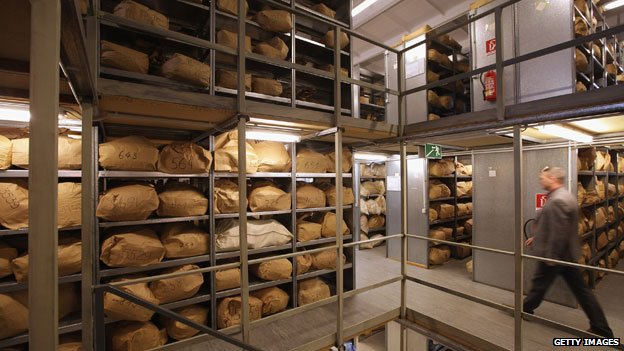
\includegraphics[width=0.9\textwidth, height=6.5cm]{stasi}
    \caption{A fraction of the 16,000 bags containing the shredded STASI archives.}
    \label{fig:stasi}
\end{figure}

\begin{figure}[H]
    \centering
    \begin{subfigure}[b]{\textwidth}
        \centering
        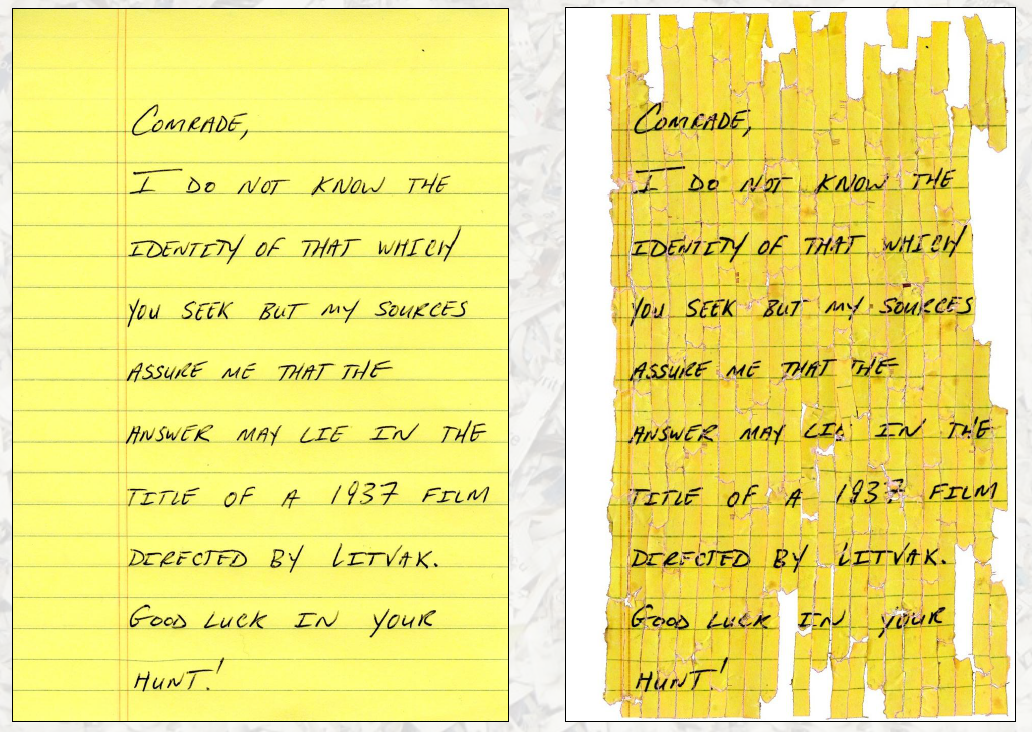
\includegraphics[width=\textwidth]{darpa1}
        \caption{One of the easiest documents in the DARPA Challenge. It is perfectly reconstructed.}
    \end{subfigure}
    ~
    \begin{subfigure}[b]{\textwidth}
        \centering
        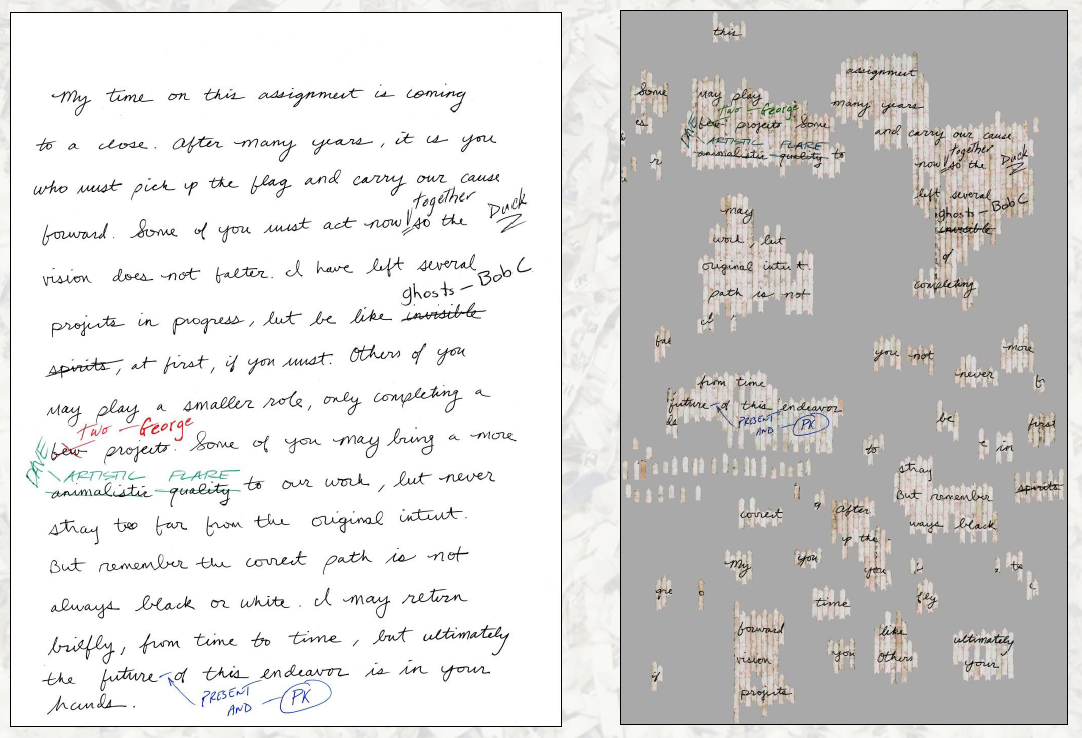
\includegraphics[width=\textwidth]{darpa4}
        \caption{One of the hardest documents in the DARPA Challenge. Even though the reconstruction is far from complete, the competitors were able to extract the information they needed from this partial solution.}
    \end{subfigure}
     \caption{Two of the DARPA Challenge documents \cite{P15}}
    \label{fig:darpa}
\end{figure}

Outside of forensics, the techniques developed to aid the reconstruction of shredded paper could also be of use to archaeologists. Several approaches to reconstructing ancient artefacts (eg: \cite{P28,P29}) face problems regarding image feature analysis and curve matching methods which are very similar to the problems tackled in shredded document reconstruction.

\section{Paper Shredders}
Paper shredders come in many different shapes, sizes and price ranges. It is therefore worthwhile to take a closer look at the types of shredders in use and at the security they offer. \\
There are 3 main categories of shredders:
\begin{itemize}
\item {\bf Strip-cut:} The cheapest and least secure variant. The paper is cut in long vertical strips. The width of the strips varies with the model.
\item {\bf Cross-cut:} The type of shredder typically used when extra security is deemed necessary. The paper is cut both vertically and horizontally into small rectangles. The size of the rectangles again varies with the model.
\item {\bf Other:} There are several types of industrial or specialist shredders that fall outside of the above categories. These include things such as \emph{Grinders} which consist of a rotating shaft with blades that grinds the paper until it is small enough to fall through a mesh. These types of shredders are rarely used outside of industrial settings, so we shall not consider them further.
\end{itemize}

The strip and cross-cut shredders can be further classified according to the DIN\footnote{Deutsche Industrial Norm} 32757 standard which is used throughout Europe \cite{P17}. This standard defines 6 common categories of strip or cross-cut shredders based on the level of security they offer, as shown in Table \ref{tab:din}.

\begin{table}[h]
  \centering
  \begin{tabular}{lllll}
    \toprule
    \multirow{2}{*}{Security Level} & \multicolumn{2}{l}{Strip-Cut} & \multicolumn{2}{l}{Cross-Cut} \\
    \cmidrule(r){2-3} 
    \cmidrule(r){4-5}
    & Shred size & No. shreds/page & Shred size & No. shreds/page \\
    \midrule
    Level 1 & 12 mm. & 18 & 11x40 mm. & 152 \\
    Level 2 & 6 mm. & 35 & 8x40 mm. & 216 \\
    Level 3 & 2 mm. & 105 & 4x30 mm. & 530 \\
    Level 4 & N.A. & N.A. & 2x15 mm. & 2100 \\
    Level 5 & N.A. & N.A. & 0.8x12 mm. & 6575 \\
    Level 6 & N.A. & N.A. & 0.8x4 mm. & 19725 \\
    \bottomrule
  \end{tabular}
  \caption{Levels of security defined by the DIN 32757 standard}
  \label{tab:din}
\end{table}

\clearpage
In order to get a better intuitive sense of these, Figure \ref{fig:dinOut} shows sample shreds outputted by machines at each level.

\begin{figure}[h]
        \centering
        \begin{subfigure}[b]{0.15\textwidth}
                \centering
                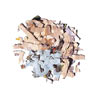
\includegraphics[width=\textwidth]{securitylevel1}
                \caption{Level 1}
        \end{subfigure}
        ~ 
        \begin{subfigure}[b]{0.15\textwidth}
                \centering
                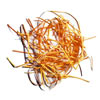
\includegraphics[width=\textwidth]{securitylevel2}
                \caption{Level 2}
        \end{subfigure}
        ~ 
        \begin{subfigure}[b]{0.15\textwidth}
                \centering
                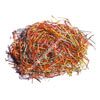
\includegraphics[width=\textwidth]{securitylevel3}
                \caption{Level 3}
        \end{subfigure}
        ~ 
        \begin{subfigure}[b]{0.15\textwidth}
                \centering
                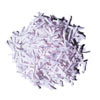
\includegraphics[width=\textwidth]{securitylevel4}
                \caption{Level 4}
        \end{subfigure}
        ~ 
        \begin{subfigure}[b]{0.15\textwidth}
                \centering
                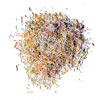
\includegraphics[width=\textwidth]{securitylevel5}
                \caption{Level 5}
        \end{subfigure}
        ~ 
        \begin{subfigure}[b]{0.15\textwidth}
                \centering
                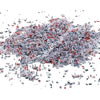
\includegraphics[width=\textwidth]{securitylevel6}
                \caption{Level 6}
        \end{subfigure}
        \caption{The output generated by shredders at the different DIN levels \cite{P17}. }
        \label{fig:dinOut}
\end{figure}

As can be seen, the amount of security offered varies drastically. At level 1 the paper could feasibly be reassembled by hand, while at level 6, the noise introduced by the cutting and scanning of the pieces would likely make a full reconstruction impossible.

\section{Roadmap}

In Chapter \ref{chap2} we formally define the problem being analysed, specify any simplifying assumptions that were made and look at the problem's complexity. In Chapter \ref{chap3} we look at previously published related work. In Chapter \ref{chap4} a novel probabilistic score function is proposed and shown to perform well in comparison with the standard cost functions used in literature. In Chapter \ref{chap5} several tractable search heuristics are analysed and a new heuristic is proposed. Chapter \ref{chap6} looks at the pre-processing function and introduces a simple and computationally efficient orientation detection method. Finally, Chapter \ref{chap7} analyses the results of the whole system and discuses possible future work.

\chapter{Problem Definition}
\label{chap2}
\section{Domain}
There are many subdomains under the general unshredding umbrella. Some of the more common distinctions look at how the paper was shredded (eg: strip-cut, cross-cut or hand torn), at the nature of the shredded document (eg: black and white or coloured; text document, picture or mixed) and at the reconstruction method (eg: fully automatic, integrated human expert or crowdsourced). 

Nowadays, most documents are mechanically shredded rather than hand torn, so we decide to focus solely on the strip-cut and the cross-cut variants. Additionally, the most commonly shredded documents are black and white, typed, text documents, so this is the variant we are interested in. Finally, we only look at fully automatic solutions, partly because previous work \cite{P1,P2} has shown that automatic methods can be modified to incorporate user interaction with relative ease.
 
\section{Assumptions}
\label{chap2Ass}
The output of a shredding device, and therefore the input to our algorithm, is a set of $n$ shreds $S = \{s_0, ..., s_{n-1}\}$. The first part of our algorithm is a pre-processing step which aims to transform the real scanned images, containing the shreds, into images we call \emph{ideal shreds}. \\
The ideal shreds have the following properties:
\begin{itemize}
\item Each ideal shred corresponds exactly to a separate image file. That is to say, an ideal shred image file will contain all the pixels belonging to a certain shred and only those pixels.
\item All ideal shreds have the same height and width.
\item All edges on all ideal shreds are either perfectly vertical or perfectly horizontal.
\item All ideal shreds are correctly orientated. That is to say, if the original document were displayed with its longest edge vertically aligned, then all ideal shreds have the same orientation they would have in that original document (note that this means the document may be ``upside down"; this is fine as long as all shreds share the same orientation).
\item The ideal shred image files contain only pure white and pure black pixels.
\end{itemize}

The problem of reducing the real shreds to these ideal shreds is analysed in Chapter \ref{chap6}. For the rest of this work, the input to the algorithm is assumed to consist of ideal shreds (see Figure \ref{fig:idealShreds}).

\begin{figure}[h]
        \setlength{\fboxsep}{-0.1cm}
        \centering
        \fbox{
        \begin{subfigure}[b]{0.079\textwidth}
                \centering
                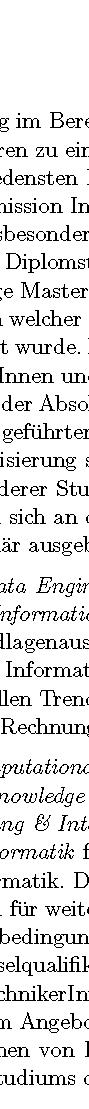
\includegraphics[width=\textwidth]{wip/wip3}
        \end{subfigure}
        }
        ~ 
        \fbox{
        \begin{subfigure}[b]{0.079\textwidth}
                \centering
                
\includegraphics[width=\textwidth]{wip/wip1}
        \end{subfigure}
        } 
        ~ 
        \fbox{
        \begin{subfigure}[b]{0.079\textwidth}
                \centering
                
\includegraphics[width=\textwidth]{wip/wip9}
        \end{subfigure}
        }
        ~ 
        \fbox{
        \begin{subfigure}[b]{0.079\textwidth}
                \centering
                
\includegraphics[width=\textwidth]{wip/wip0}
        \end{subfigure}
        } 
        ~ 
        \fbox{ 
        \begin{subfigure}[b]{0.079\textwidth}
                \centering
                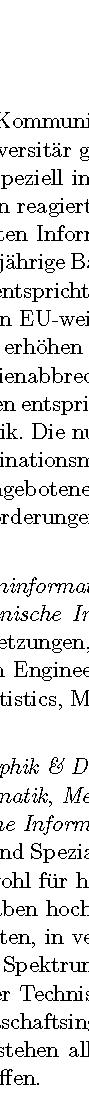
\includegraphics[width=\textwidth]{wip/wip7}
        \end{subfigure}
        } 
        ~ 
        \fbox{ 
        \begin{subfigure}[b]{0.079\textwidth}
                \centering
                
\includegraphics[width=\textwidth]{wip/wip5}
        \end{subfigure}
        } 
        ~ 
        \fbox{ 
        \begin{subfigure}[b]{0.079\textwidth}
                \centering
                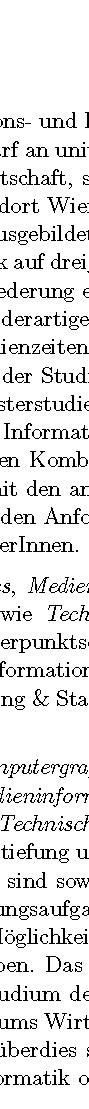
\includegraphics[width=\textwidth]{wip/wip6}
        \end{subfigure}
        } 
        ~ 
        \fbox{
        \begin{subfigure}[b]{0.079\textwidth}
                \centering
                
\includegraphics[width=\textwidth]{wip/wip4}
        \end{subfigure}
        } 
        ~ 
        \fbox{ 
        \begin{subfigure}[b]{0.079\textwidth}
                \centering
                
\includegraphics[width=\textwidth]{wip/wip8}
        \end{subfigure}
        } 
        ~ 
        \fbox{ 
        \begin{subfigure}[b]{0.079\textwidth}
                \centering
                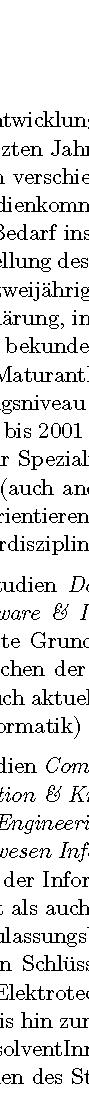
\includegraphics[width=\textwidth]{wip/wip2}
        \end{subfigure}
        }
        \caption{Example of \emph{ideal shreds} of a document. }
        \label{fig:idealShreds}
\end{figure}

Now that we have our ideal shreds, the problem can be further subdivided into two functions.

\section{Formal definition of score and search functions}
\textbf{The edge scoring function:} This first function analyses all pairs of shreds for edge matches and returns a number that represents the quality of each match (see Figure \ref{fig:edgeMatch}).

\begin{figure}[h]
    \centering
    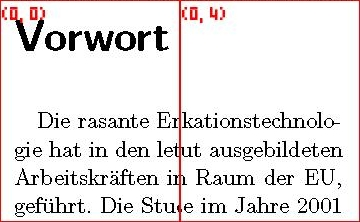
\includegraphics[width=0.8\textwidth]{conf}
    \caption{A potential edge between two shreds. The edge scoring function has to evaluate this match and report how good it is.}
    \label{fig:edgeMatch}
\end{figure}

Formally, we must obtain: $sc_r(s_i, s_j)$ and $sc_b(s_i, s_j), \forall s_i, s_j \in S $ where  $sc_r(s_i, s_j)$ is the score of placing $s_j$ to the right of $s_i$ and $sc_b(s_i, s_j)$ is the score of placing $s_j$ below $s_i$.

\textbf{The global search function:} The second function receives the scores between all pairs of shreds as input and must find an arrangement of shreds in 2D space that optimises the global score.

We consider the global score to be the sum of all individual scores between neighbouring shreds. Modifying the formulation made in \cite{P20}, we can define a solution of the search function as a mapping $ \Pi : D^2 \rightarrow S$ where $D = \{0, ..., |S|-1\}$. This means each position in a two dimensional space defined by $D^2$ corresponds to a shred. Formally
\[
\Pi(r,c) =
\left\{
	\begin{array}{ll}
		\mbox{the shred placed at row r, column c; IF such a shred exists } \\
		\mbox{a completely blank shred; OTHERWISE }
	\end{array}
\right.
, \forall r,c \in D \]

The global score of a shred placement, $GS(\Pi)$ can then be defined as:\footnote{This assumes the shreds are indexed such as $(0,0)$ is the top, leftmost shred and $(|S-1|,|S-1|)$ is the bottom, rightmost shred} \[GS(\Pi) = \sum_{r=1}^{|S|-1} \sum_{c=1}^{|S|-1} (sc_b(\Pi(r-1,c),\Pi(r,c)) + sc_r(\Pi(r,c-1),\Pi(r,c)))  \]
 
\section{Complexity}
The scoring function is forced to calculate a score for each pair of shreds. Therefore, if we have $n$ shreds, we will have to calculate on the order of $n^2$ scores. Looking at the number of pieces that a page can be shred into (Table: \ref{tab:din}), we can see that this quickly becomes a problem. Some techniques that could mitigate this bottleneck are explored in Section \ref{chap3PP}

The search function, on the other hand, has to search the space of all possible two dimensional placements of edges. Since we have no information about the original shape of the document, the space we must consider for $n$ shreds will have $length = height = n$ and therefore $positions = n^2$. This means we are placing $n$ shreds into $n^2$ slots and so the number of possible placements is $\displaystyle {n^2 \choose n} = \frac{n^2!}{n!(n^2-n)!} $. Clearly this is a huge search space and, in fact, \cite{P1} has shown that the search problem is NP-hard even if restricted to just strip-cut documents. Again, looking at Table \ref{tab:din} we can easily see that optimal search solutions are not feasible for this problem and we must therefore make do with heuristics.

\section{Modularity}
By splitting the reconstruction into the three mentioned sub-functions (pre-processing, score and search), we attempt to solve the problem in a modular way.

Any of the three functions could be enhanced, or replaced entirely without needing to make any modifications in the other two functions. This is particularly useful since each function has quite a different goal and utilises different techniques (for instance, all optical character recognition related algorithms will be restricted to the score function). This separation of concerns allows us to improve algorithms more easily or extended them to different problem domains. 

This modularity is something that was aimed at throughout, so that not only can any of the functions be replaced, but they can easily be composed with other functions. These factors will be discussed more thoroughly in the chapters corresponding to each function.

\chapter{Literature Review}
\label{chap3}

\section{Related Problems}
The unshredding problem can be viewed as a special case of the general jigsaw reconstruction problem. Automatically solving jigsaws has been an active area of research since the 60s \cite{P21} and as such there is a wealth of information published on this topic. However the majority of early methods focus entirely on the shape information of the pieces (eg: \cite{P21,P22}) and are therefore not applicable to our problem. More recently there have been several attempts that also utilise the visual information of the pieces (eg: \cite{P23,P24}), however these methods mostly focus on the distribution of colours on the images and thus are not easily applicable to our black and white domain. Additionally, the solutions proposed are generally restricted to very small problem instances (usually less than 50 pieces), which is too small a number for our purposes. One promising method is presented in \cite{P25}. Here the authors reconstruct the jigsaw while looking only at image features, and also manage to solve instances with as many as 320 pieces. The features used in their comparison function are viable candidates for shred comparison or clustering.

Another related problem is the reconstruction of full-colour shredded documents. As opposed to the jigsaw puzzle formulation, this problem has no edge shape information to use. However, the availability of full-colour means that the amount of information available on a shred is much higher than in the case of binary data (i.e. black and white pixels). A thorough review of this problem is presented in \cite{P26}. Here, Skeoch analyses several types of distance functions that look at how similar two pixels are and uses these to design some simple yet effective shred comparison functions. However, the author notes that these methods don't work very well on black and white documents. Additionally, the analysis is restricted to the strip-cut variant.

Yet another related problem, is the reconstruction of hand-torn documents. In this problem, edge shape becomes once more a big factor, especially since hand-torn documents tend to contain much fewer shreds than mechanically torn ones. Most approaches (eg: \cite{P18,P27,P31}) focus on curve matching methods and are therefore not applicable to us. Additionally, since the search space is smaller, such approaches are generally quite computationally expensive (\cite{P18}, for instance, was only tested on up to 15 shreds). One interesting method in this area was presented by De Smet in \cite{P30}. Here, he proposes a search algorithm that takes advantage of the way humans tend to stack hand-torn shreds and which successfully manages to speed up the search process. A method more applicable to our problem is analysed in \cite{P32}, where the authors look at the effectiveness of different features when used to cluster the shreds based on similarity.

A final related problem is the \emph{semi-automatic} reconstruction of shredded documents. Some of the most successful reconstruction methods developed so far, including those that won the DARPA Shredder Challenge \cite{P33,P34} fall under this category and incorporate human input into the evaluation loop. Using even a small amount of human expertise can vastly reduce the difficulty of the problem, because humans can catch errors early, before these have a chance to propagate. One example of such a system is shown in Figure \ref{fig:deshredder}

\begin{figure}[h]
    \centering
    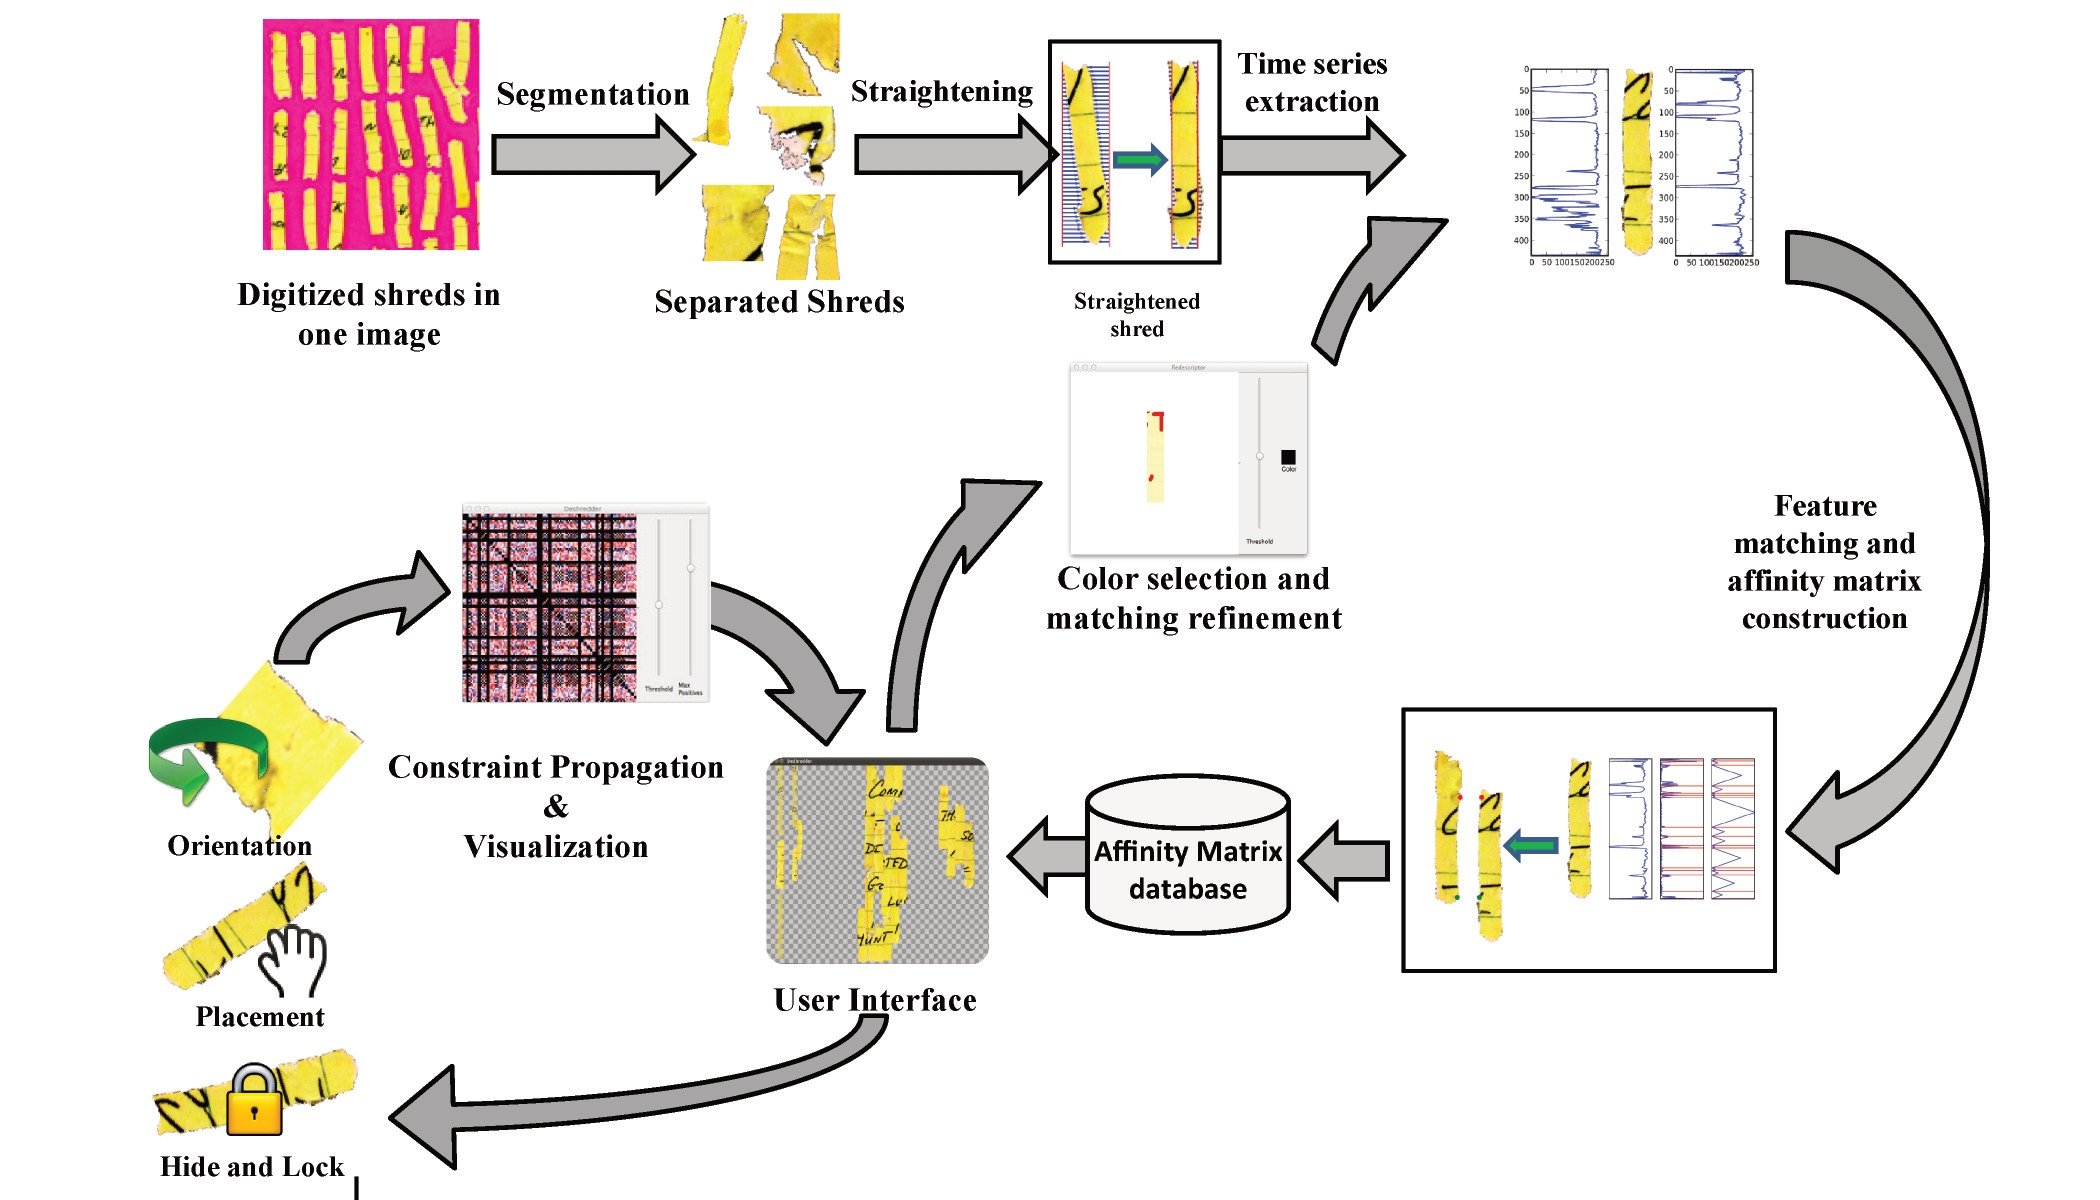
\includegraphics[width=\textwidth]{deshredder.jpg}
    \caption{The pipeline of the Deshredder algorithm and user interface. Figure taken from \cite{P34}.}
    \label{fig:deshredder}
\end{figure}

A particularly interesting semi-automatic approach was developed in \cite{P35}, where the authors show a shred to the user and then allow him to draw what a portion of the neighbouring shred might look like. The user is then shown shreds which match his drawing, at which point he can either select a correct match from the proposed edges or decide change his drawing.

\clearpage

\section{Edge comparison functions}
Most previously published approaches have used a \emph{cost} function to compare edge matches. A cost function means that a lower cost represents a better match and, in particular, a cost of $0$ shows a perfect match and a cost of $\infty$ shows an impossible one. 

Relatively little progress has been made in developing the cost function. Most papers (eg: \cite{P1,P5,P6,P7,P20,P36}) settle on a simple ``Gaussian cost" formulation which does a weighted difference of each pair of adjacent pixels on either side of the proposed join and increases the cost of the join if the pixels are too dissimilar. The logic here is that neighbouring shreds are more likely to have matching pixels on their edges. In order to mitigate the effect of noise, a ``Gaussian" comparison is done by looking at a small neighbourhood of pixels rather than doing a single pixel to pixel comparison (see Figure \ref{fig:gausIdea}).

\begin{figure}[h]
    \centering
    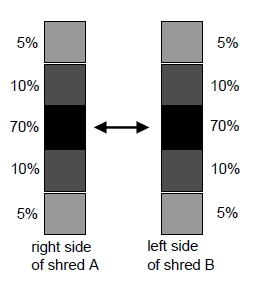
\includegraphics[width=0.5\textwidth]{gausIdea}
    \caption{Cost function calculating the weighted sum of the difference between two opposing pixels and their respective opposing neighbours. Figure taken from \cite{P20}}
    \label{fig:gausIdea}
\end{figure}

In order to formally define this function, we first must get a term for the weighted sum of the $y$th pixel on shred A being matched to the corresponding $y$th pixel on shred B. We call this function $e'_h(A,B,y)$ and define it as: 
\begin{equation*}
\begin{split}
e'_h(A,B,y) = &  |0.7(v_r(A,y) - v_l(B,y)) + \\ 
              &  0.1(v_r(A,y+1) - v_l(B,y+1)) + \\
              &  0.1(v_r(A,y-1) - v_l(B,y-1)) + \\
              &  0.05(v_r(A,y+2) - v_l(B,y+2)) + \\
              &  0.05(v_r(A,y-2) - v_l(B,y-2))|
\end{split}
\end{equation*}
where $v_r(A,y)$ returns the $y$th pixel on the right edge of shred $A$ and $v_l(A,y)$ returns the $y$th pixel on the left edge of shred $A$.

Once we have this weighted sum, we can pass it through a threshold $\tau$ in order to obtain the pixel cost: 
\[ e_h(A,B,y) = \left\{
	\begin{array}{ll}
		1 \mbox{ if } e'_h(A,B,y) \geq \tau \\
		0 \mbox{ otherwise }
	\end{array}
\right. \]

And finally, the edge cost is simply the sum of all pixel costs:
\[c_r(A,B) = \sum_{y \in \mbox{\small Edge Pixels}} e_h(A,B,y) \]

One problem with the above formulation is that matching a completely white edge to another completely white edge will give a perfect cost of 0. Therefore whenever such a white-on-white match is available it will be taken, which can result in undesirable behaviour (see Figure \ref{fig:white}).

\begin{figure}[h]
    \centering
    
\includegraphics[width=\textwidth]{white}
    \caption{{\bf Left:} the correct match. {\bf Right:} white-on-white match which would get a perfect cost under the Gaussian cost function and be incorrectly preferred}
    \label{fig:white}
\end{figure}

A refinement to the cost function that solves the white-on-white problem is proposed in \cite{P2}. Here, the authors base the cost only on how well the black pixels match (i.e they disregard matching white pixels from their cost computation). This paper also introduces a heuristic that penalises edges that have too few black pixels on them. These improvements result in the best cost function published so far and therefore the main benchmark against which we will compare our method. 

The authors of \cite{P8} present another proof-of-concept cost function improvement. They use computer vision techniques to identify individual characters that were split between different shreds and try to match them together. The authors learn the correct character shapes from the shreds themselves, therefore the method can be applied on any character set. The paper has promising preliminary results but doesn't provide comparisons with other cost functions, so aspects such as robustness to noise remain unclear.

\clearpage
\section{Search functions}
\label{chap2Search}
Significant effort has been made towards finding a good search function and several different approaches have been explored.  In \cite{P1}, the authors show that the search problem is NP hard by reducing it to a Travelling Salesman Problem. The authors then solve this Travelling Salesman Problem by using the Chained Lin-Kernighan heuristic \cite{P37}.  In \cite{P6} an exact solution is attempted via Integer Linear Programming. Due to the large search space, this paper only looks at the strip-cut variant. The method presented here yields very good results but is intractable for any number of strips above 150. This suggests that any attempts to use Integer Linear Programming for the cross-cut variant would likely be futile. 

Several attempts at using top-down local improvement have also been made. These methods first obtain a seed solution using a heuristic function and then attempt to improve upon this solution via local search methods. In \cite{P5} the authors apply the Variable Neighbourhood Search meta-heuristic \cite{P38}, which contains two parts, a local search function called variable neighbourhood descent and a perturbation function which aims to help the local search escape local optima. The variable neighbourhood descent searches neighbourhoods of increasing size for a solution that is better than the current one. Here neighbourhoods are obtained by either swapping single pieces, or shifting groups of pieces around. The perturbation function simply adds some randomness in the form of occasionally switching the solution to a neighbour even if the neighbour's score is worse than our current score. In the same paper, the authors also define an Ant Colony Optimization solution \cite{P39}. This Ant Colony Optimization formulation proved to be overall better than the Variable Neighbourhood Search heuristic, but at the cost of a longer runtime. These results are improved upon in \cite{P7}, where the authors use the same Variable Neighbourhood Search formulation, but embed it into a genetic algorithm. The method defines several mutation and recombination operators which are applied to an initial population of solutions generated by some simple heuristics. Between every step of the genetic algorithm, the solution pool is improved by running the Variable Neighbourhood Search algorithm.

As mentioned above, \cite{P5,P7} both rely on heuristic search methods to provide them with initial seed solutions. One of these methods is the Row Building Heuristic (RBH). RBH tries to take advantage of the fact that shreds with a completely white edge probably belong on the margin of the document. RBH therefore randomly selects a shred with a white left edge as its starting shred. It then adds the best match, as defined by the cost function, to the right of this starting edge. The greedy process is repeated, thus increasing the length of the current row, until we append a piece which has a white right edge, at which point the algorithm simply restarts and attempts to build the next row. 

The second heuristic worth mentioning is the Prim Based Heuristic, which is analogous to the Prim minimum spanning tree algorithm \cite{P40}. This works by picking a random shred as a starting point and then expanding it by adding a shred to one of the four possible neighbouring positions. The process is repeated, always greedily adding the best edge to one of the neighbours of our current solution (see Figure \ref{fig:prim}). 
\begin{figure}[H]
        \centering
        \begin{subfigure}[b]{0.45\textwidth}
                \centering
                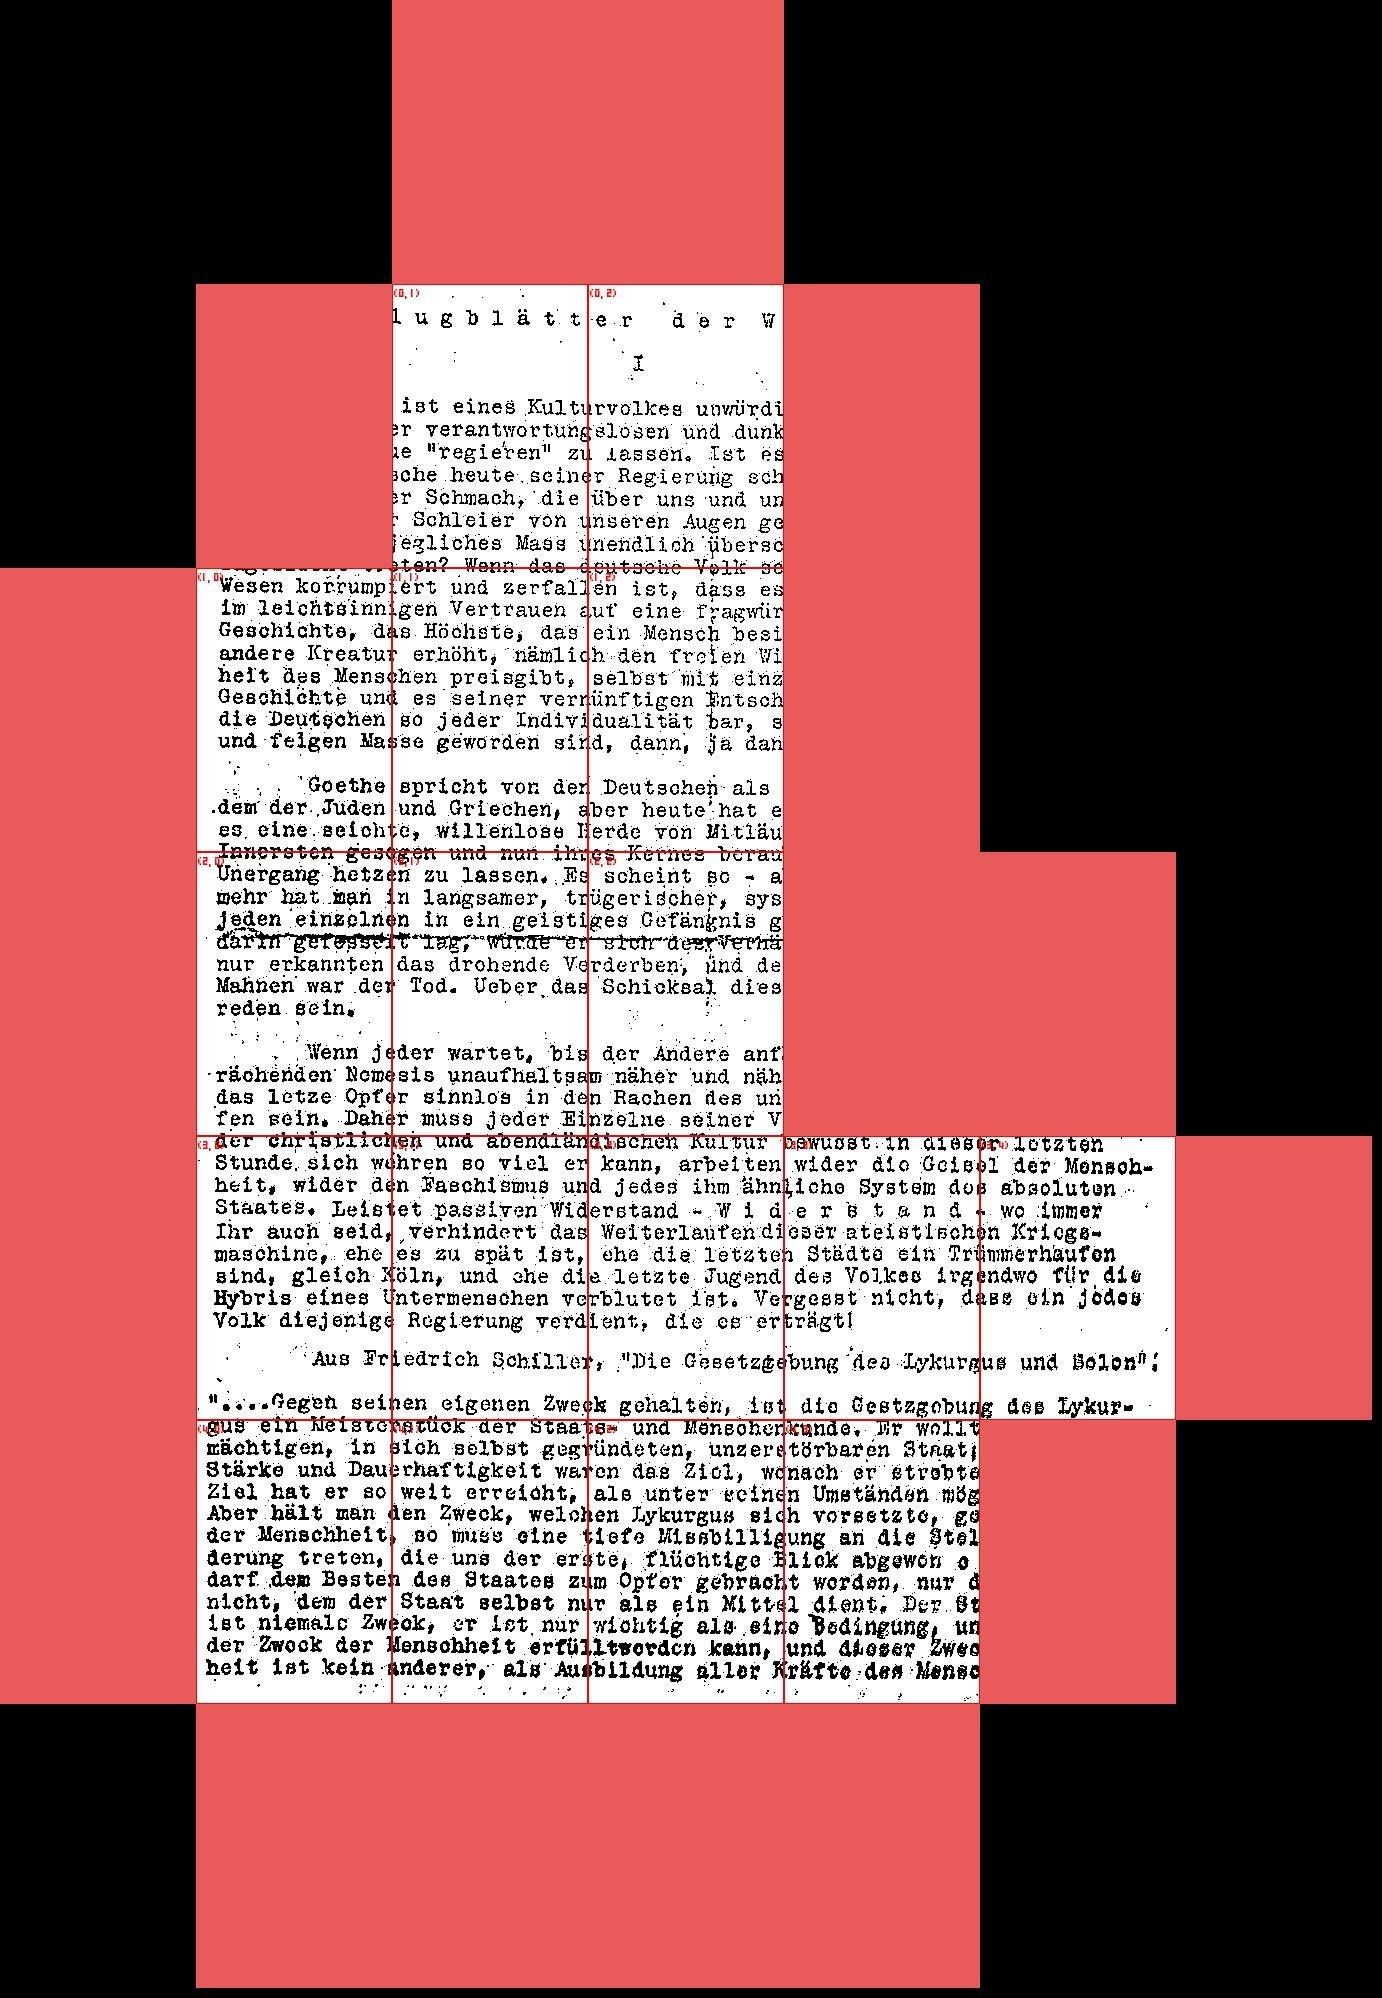
\includegraphics[width=\textwidth]{prim1}
                \vspace{0.3em}
        \end{subfigure}
        ~ 
        \begin{subfigure}[b]{0.45\textwidth}
                \centering
                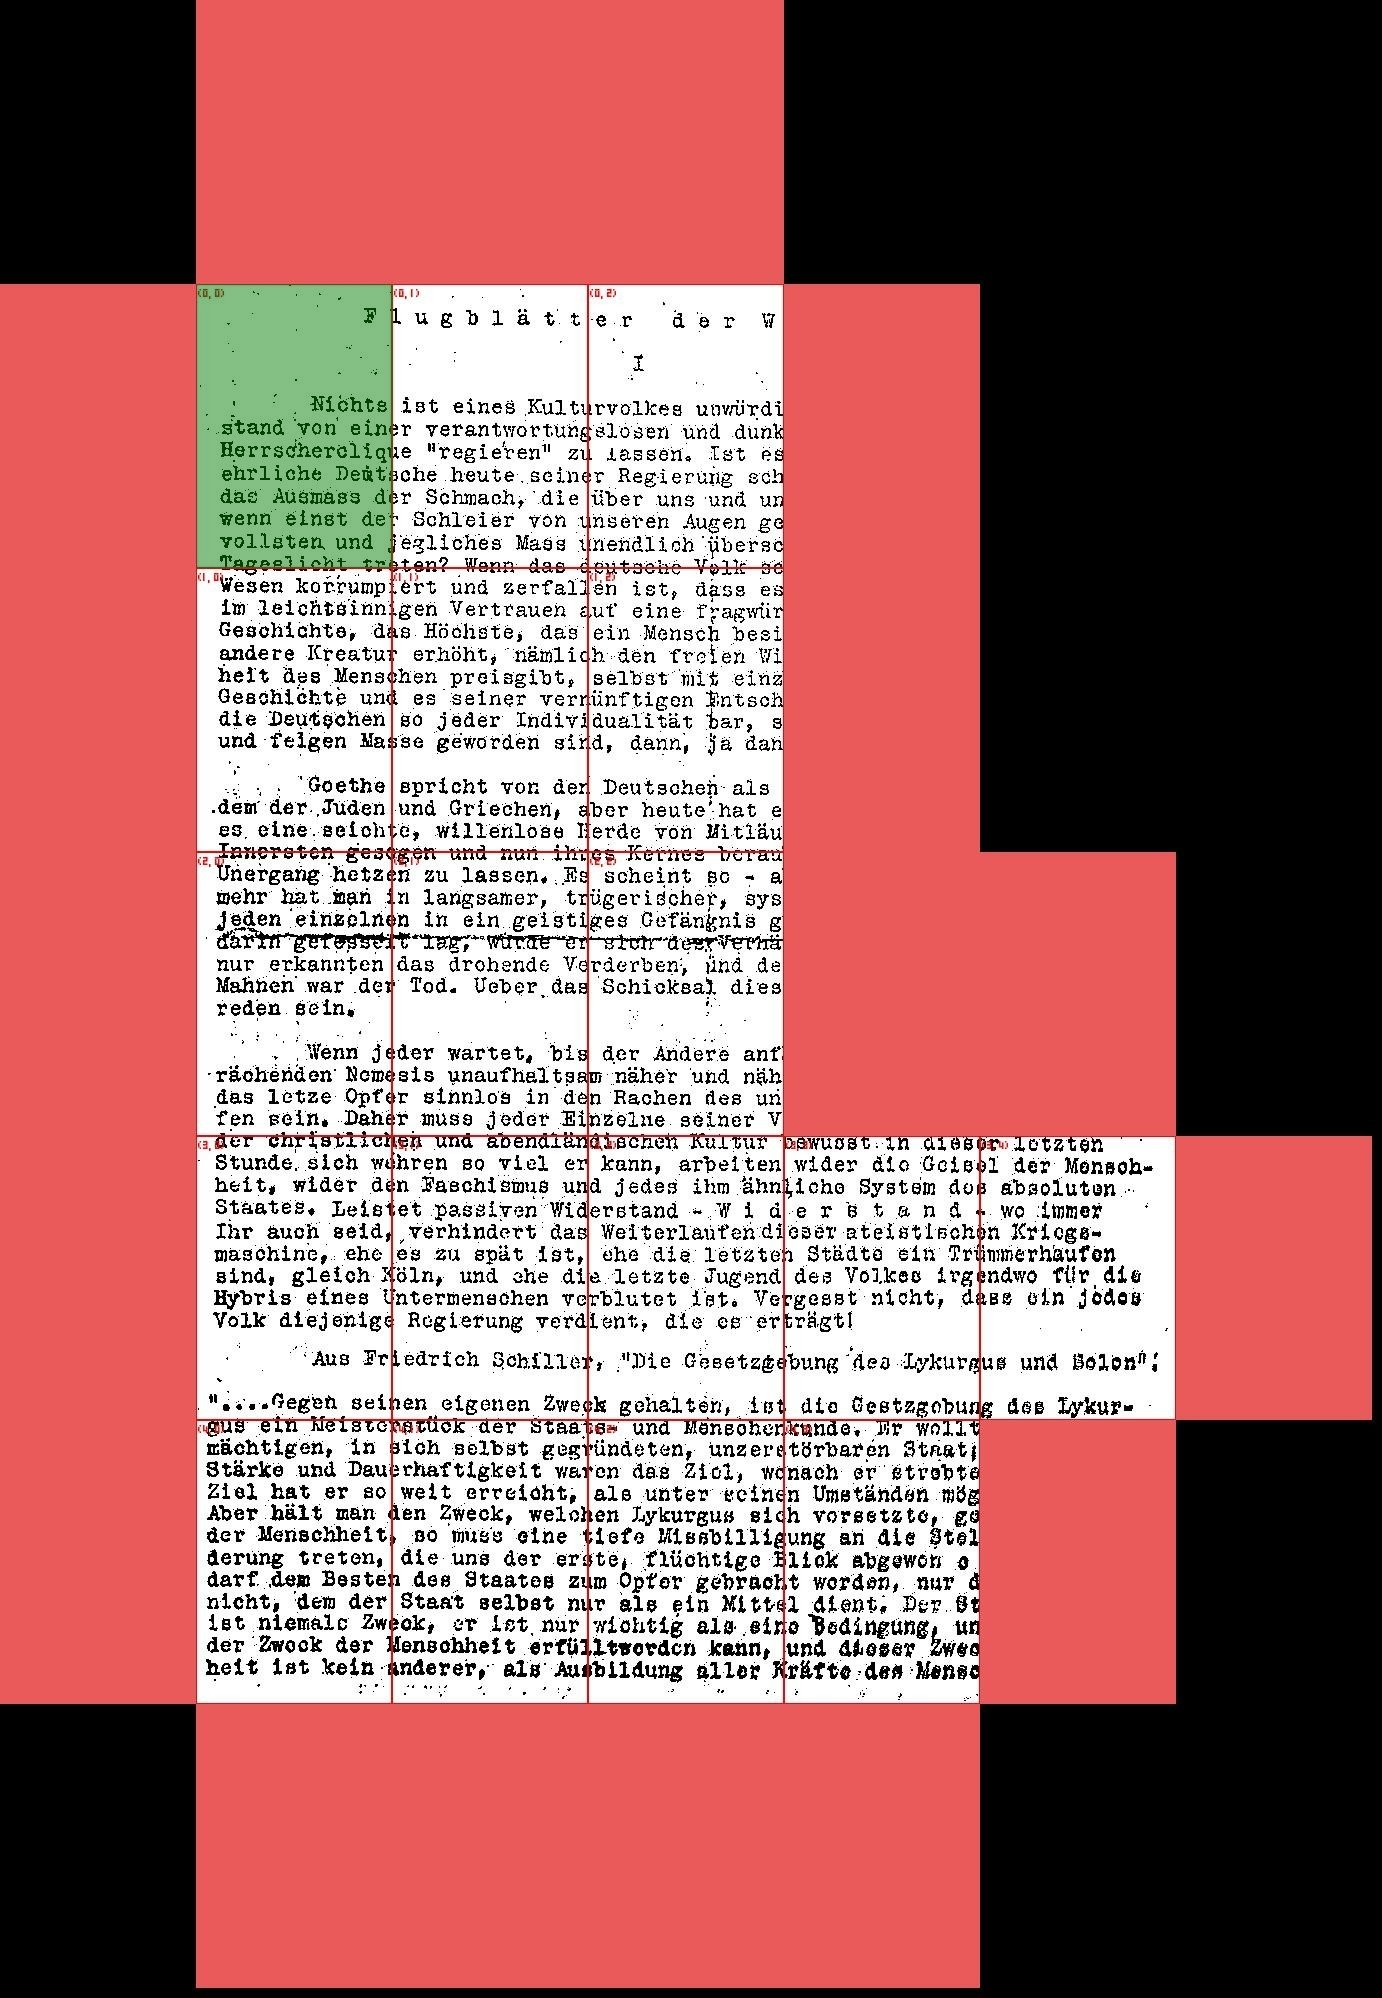
\includegraphics[width=\textwidth]{prim2}
                \vspace{0.3em}
        \end{subfigure}
        ~ 
        \begin{subfigure}[b]{0.45\textwidth}
                \centering
                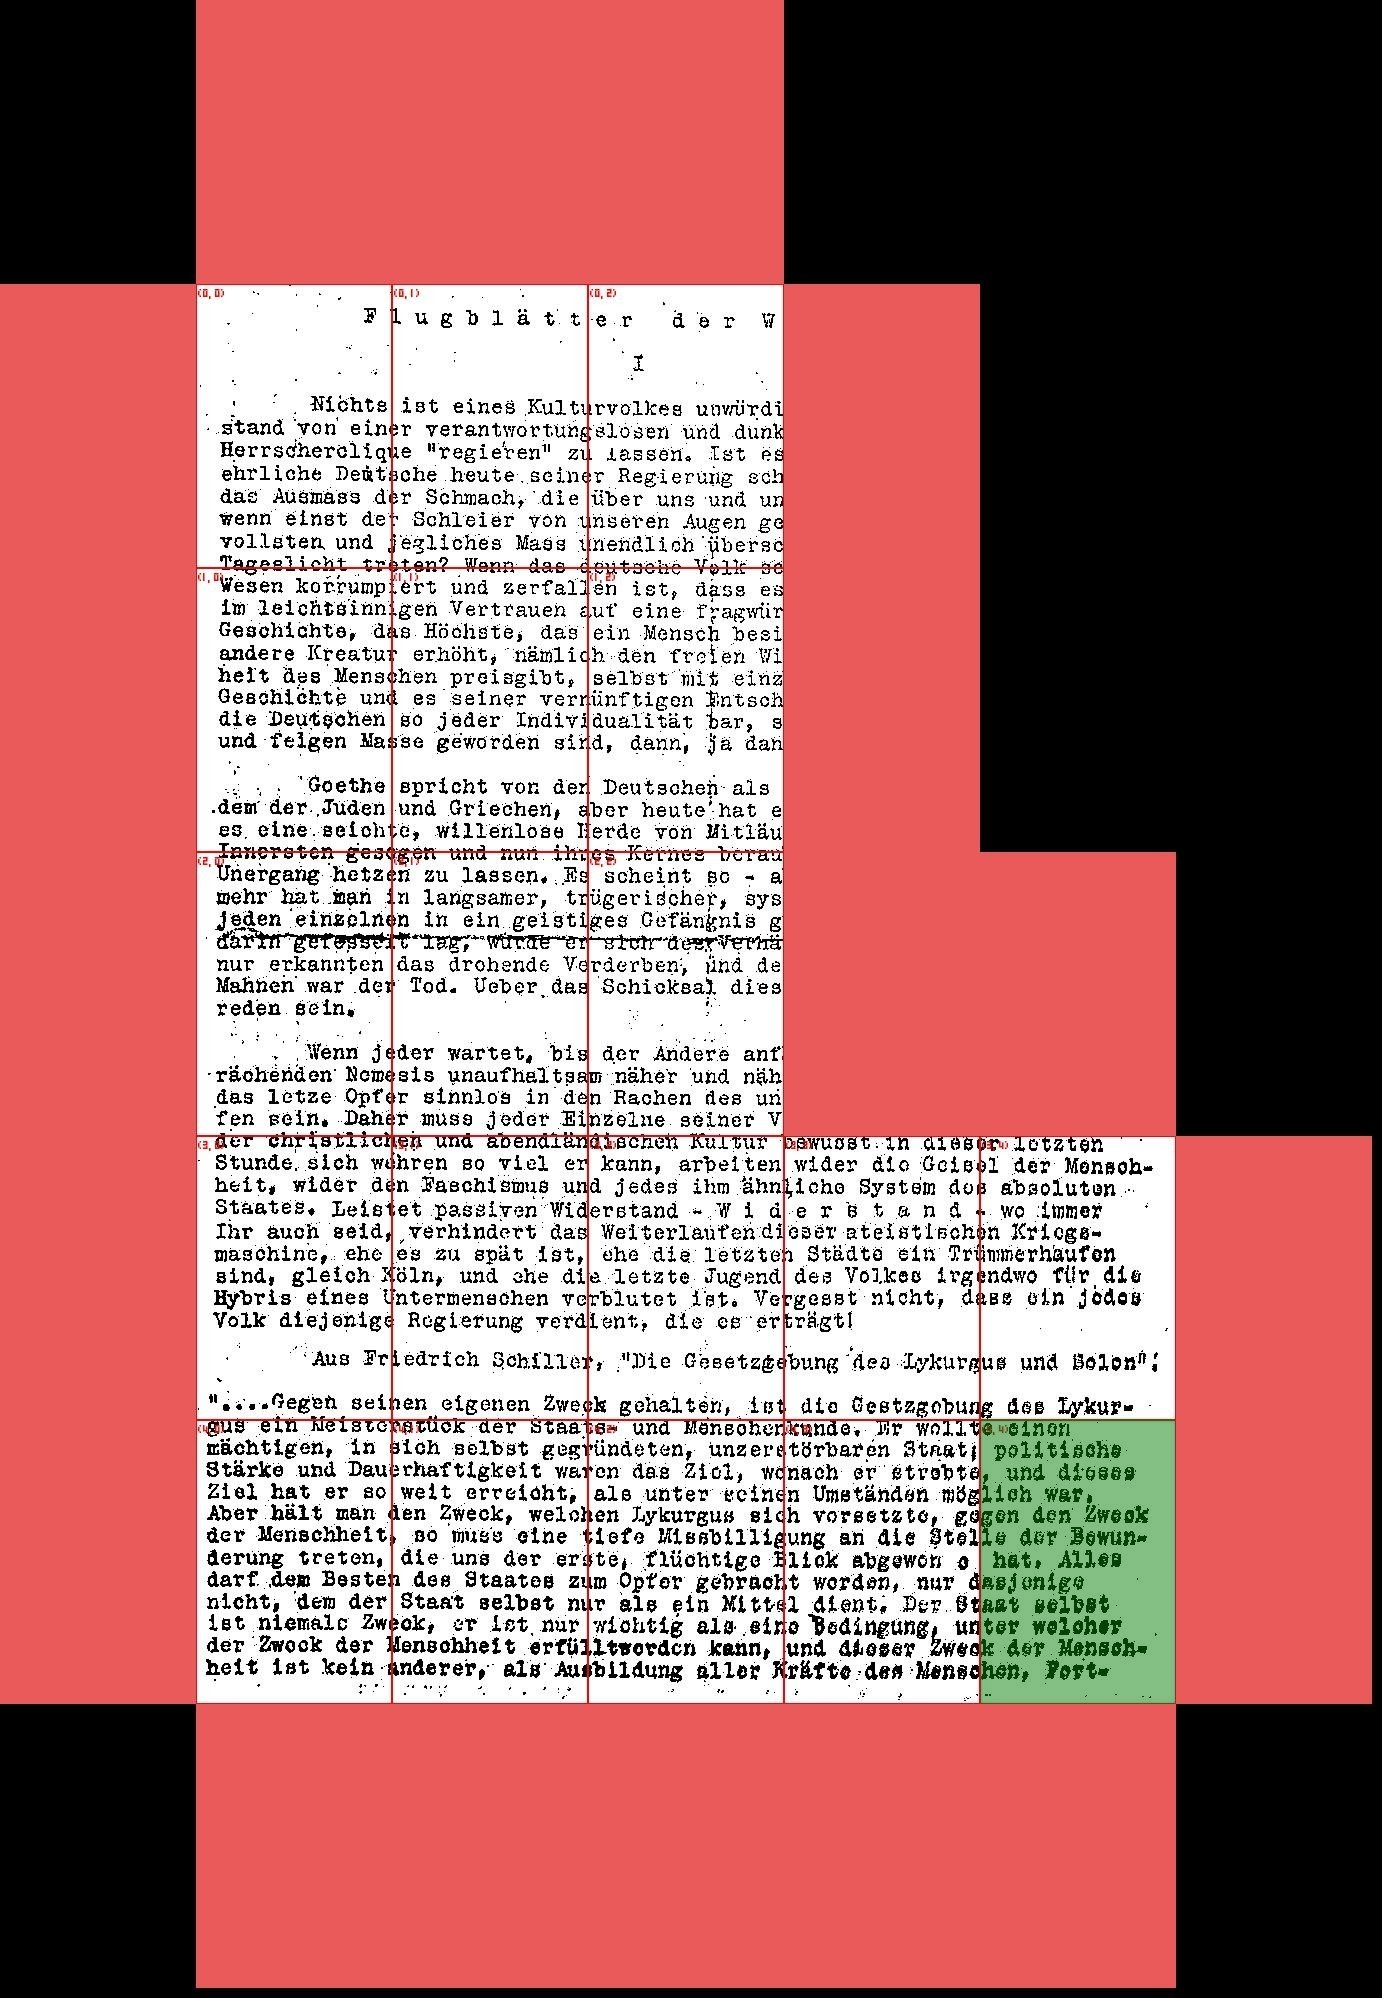
\includegraphics[width=\textwidth]{prim3}
        \end{subfigure}
        ~ 
        \begin{subfigure}[b]{0.45\textwidth}
                \centering
                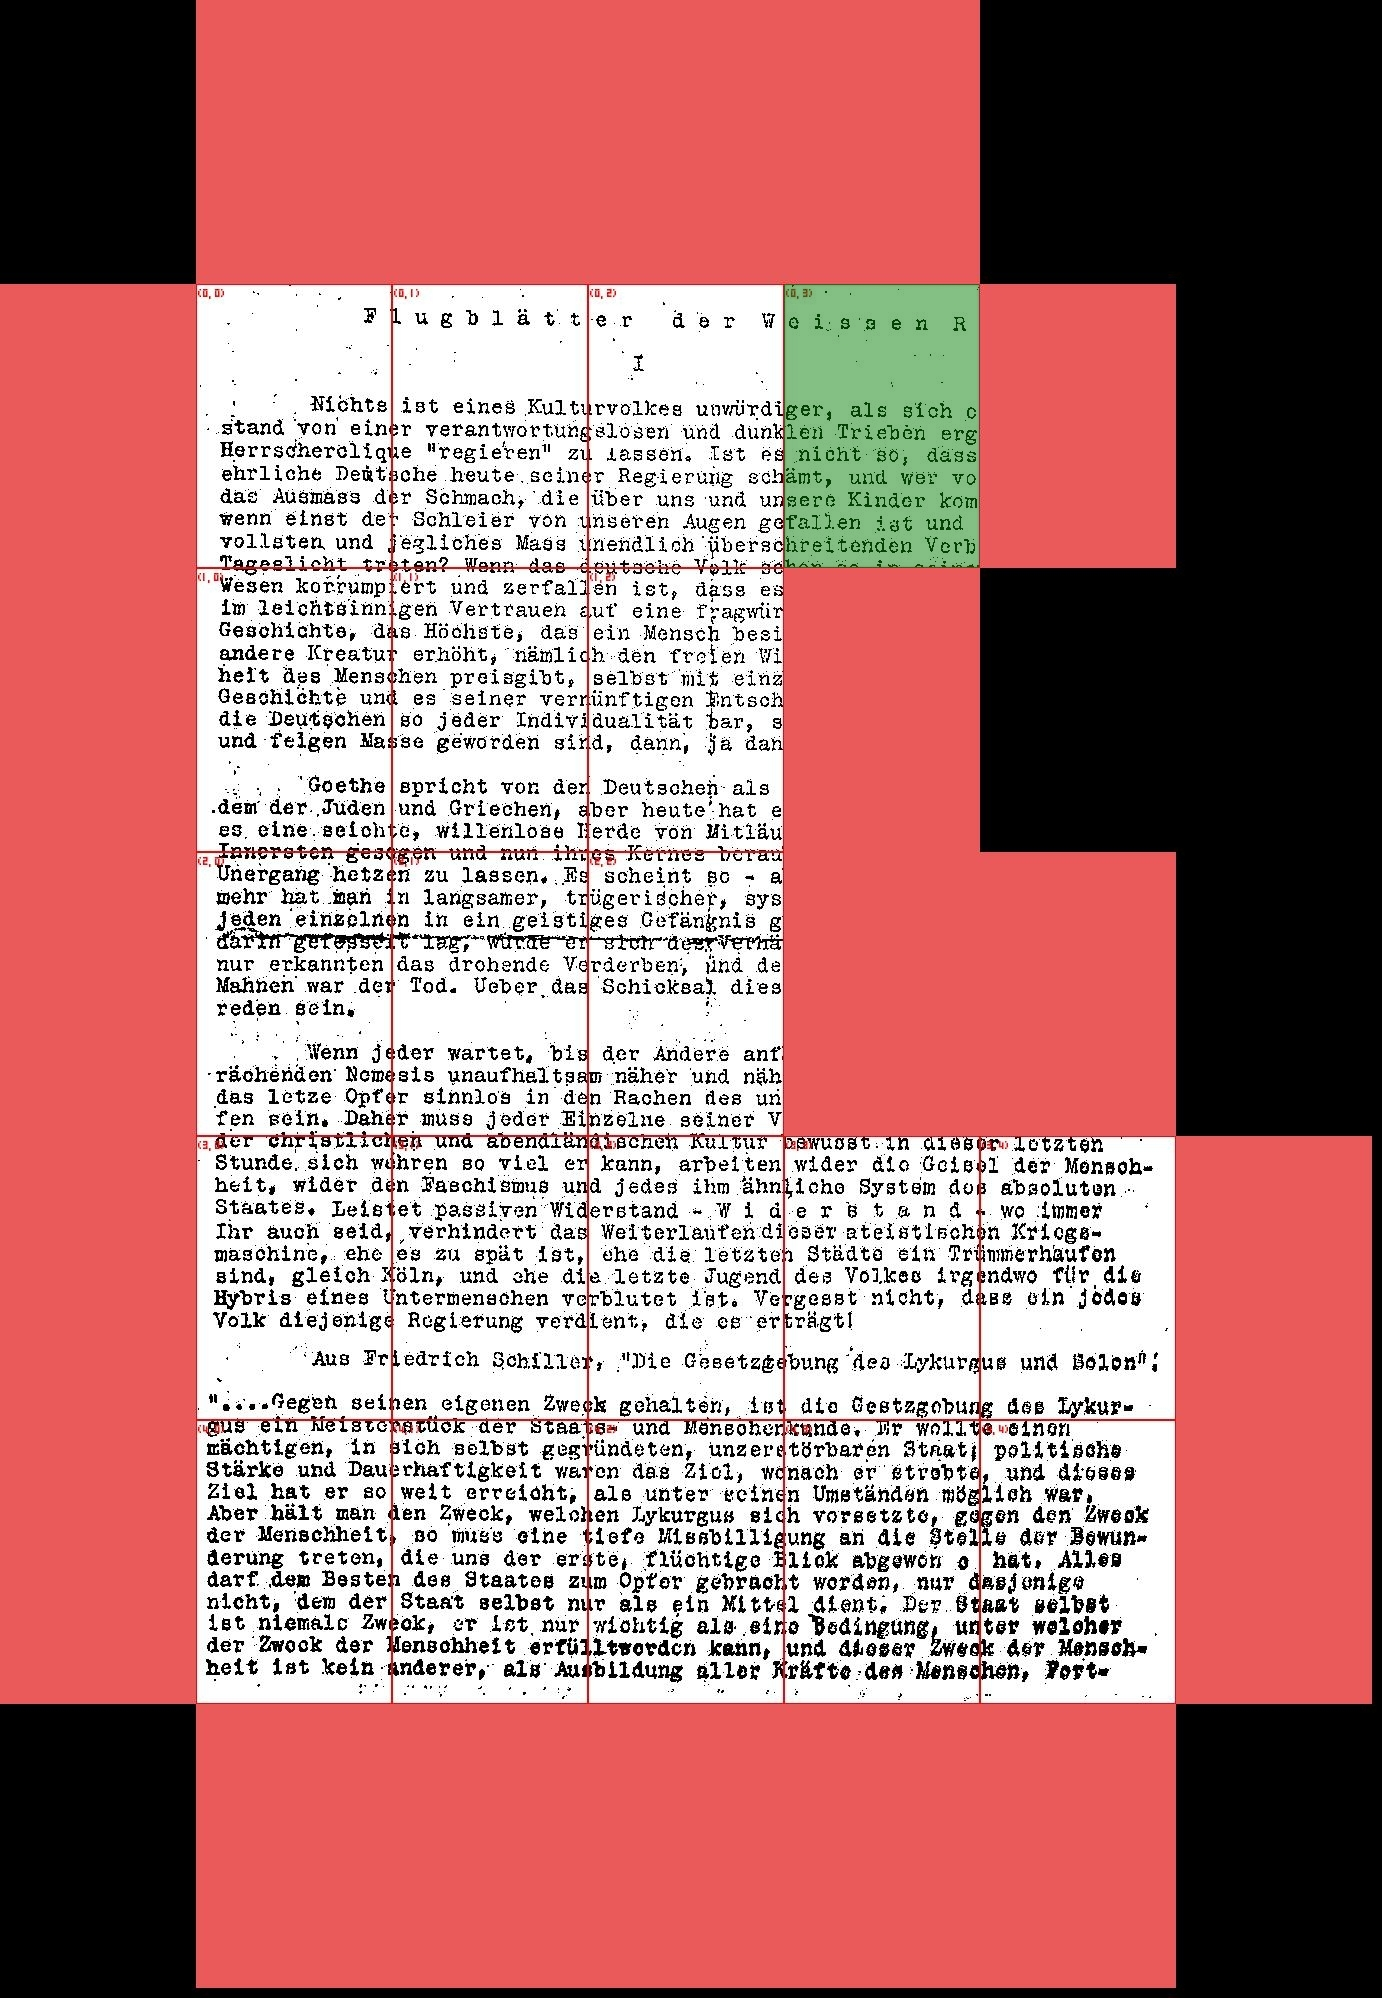
\includegraphics[width=\textwidth]{prim4}
        \end{subfigure}
        \caption{Four steps from the middle of a Prim search are shown. The green pieces highlight the changes that occur in every step and the red pieces show the positions that are considered for the insertion of new shreds.}
        \label{fig:prim}
\end{figure}
Lastly, a heuristic called \emph{ReconstructShreds} is proposed in \cite{P2}. This heuristic can be viewed as a relaxation of the Prim heuristic such that we can have multiple clusters of pieces at any time. ReconstructShreds is looked at in more detail in Section \ref{chap5Desc}.

\section{Pre-processing the shreds}
\label{chap3PP}
As discussed in Section \ref{chap2Ass}, a pre-processing step is needed in order to transform the real, noisy, input into a form suitable for the rest of the algorithm. Several aspects of this pre-processing step have been previously analysed in literature, namely: segmentation, skew correction, up/down orientation and clustering.

\textbf{Segmentation:} The first issue is to actually extract the shreds from the scanned image and to make sure they're all the same size. Skeoch \cite{P26} tackles this problem by first thresholding the original image as to detect the position of the pixels sufficiently different from the background colour. Several ways of automating the threshold selection method are analysed but ultimately, due to the high variance present in scanned images, user input is still required. After thresholding, Skeoch fits rectangles to all pixel blobs over a certain size and thus obtains the individual shreds. A complication can arise when processing narrow strip-cut documents as the shreds can have a tendency to curve, in a manner similar to human hair. Since this curvature can trip up the rectangle fitting, Skeoch proposes instead to detect the corners of the shreds and then fit a polynomial to the edges. An alternative that may be preferable if noise is a major issue, would be to use the Generalised Hough Transform \cite{P44} to detect the delimitation of each shred.

\textbf{Skew Correction:} If we have already detected the shred's bounding rectangles, then fixing the skew of the image can be done by rotating the rectangles so that their longest side is vertical. Alternatively, in \cite{P34} the authors take a different approach by fixing the skew first. They frame the skew correction as an optimization problem and seek the rotation that would minimize the distance between each shred pixel and a vertical line. This completely avoids the need to fit or detect the lines of the shreds since, after the shred has been oriented vertically, a simple bounding box can be taken around it. Both approaches work reasonably well in practice, with maximum errors in the range of 1-2 degrees.

If accuracies greater than this are required, then more complex document orientation methods can be employed. For instance, in \cite{P41}, the authors use a row detection method and then predict the skew and orientation based on some features of these rows. Their method has a precision of 0.1 degrees, and similar results have also been obtained by several other algorithms (eg: \cite{P42,P43}). However none of these methods have been tested on extremely small shreds. Their performance degradation as the information on a shred decreases is unclear and may pose a problem.

\textbf{Up/Down Orientation:} If we have opted for the simpler methods of performing skew correction, then the shreds will now be either correctly oriented or rotated by 180 degrees. Several reliable methods have been developed to deal with this problem. If we restrict the problem to documents written in Roman script, then a robust method is presented in \cite{P45}. The author obtains 100\% accuracy even on documents degraded by noise. Additionally, the method is employed for shred orientation detection in \cite{P32}, thus showing the method can handle orientation on smaller pieces of text (though that paper handles hand-torn documents, so the shreds they look at aren't as small as the ones we might be interested in). For a completely general approach, there are also several orientation methods that work on both Roman and non-Roman scripts, usually by employing some learning algorithm (eg: \cite{P46})

\textbf{Clustering:} One last pre-processing task, useful in some domains, involves clustering the shreds. The problem is that often the shreds of many different documents will be mixed together, thus making the reconstruction process intractable. However, if not all the documents are completely uniform, then the search space can be reduced by clustering the shreds into similar document classes. Several image features have been proposed for this classification task. In \cite{P47}, the authors propose the use of the MPEG-7 standard descriptors \cite{P48} and look at the effectiveness of features such as colour, shape and texture. The paper shows encouraging results for coloured pages, but black and white documents prove to be a harder problem. Their method is expanded upon in \cite{P49}, where in addition to the MPEG-7 descriptors, the authors also detect higher level features, such as whether the paper is from a notebook, by using the Hough transform \cite{P50}. In \cite{P32} the authors propose several other custom features, such as detecting whether the text is typed or handwritten and detecting the type of paper used. For text documents, good results are obtained if the text or paper colour varies, or if the writing changes from typed to handwritten. Making use of subtler features, such as differences in fonts, proved to be more difficult.

\chapter{Probabilistic Score}
\label{chap4}
This paper proposes a departure from the previous cost function definitions, looking instead at using a probabilistic model to directly estimate the likelihood of two edges matching.
\section{Motivation}
A pervasive problem with the cost functions discussed above is that their design is ad hoc and relies on hand-picked values based on the authors' empirical observations. For instance, in \cite{P1} the authors have to decide on the size of the Gaussian window they employ, on the weights to assign to the pixels that fall within that window and on a suitable value for their threshold function. All these parameters are given a static value but, since they are dependent on the source document, the authors would need to manually find different values for each class of documents. In \cite{P2} the authors not only face all of the above problems, but also have to decide on a threshold value for their row comparison and on another threshold regarding the minimum amount of black pixels that an edge must have in order for its matches to be considered relevant. 

This ad-hoc formulation suffer from several impediments which the probabilistic method manages to avoid or at least ameliorate: \\
\begin{table}[H]
  \centering
  \begin{tabular}{p{0.5\textwidth} | p{0.5\textwidth}}
  \toprule
  Cost function & Probabilistic score function \\
  \midrule
Relies on the values the authors hand-picked for their particular dataset. & Learns a new document's pixel distribution by analysing the shreds it is given.\vspace{1.5em} \\
Cannot be easily combined with a different similarity function. & Can be easily composed with any similarity function that produces a probability. Several such functions already exist, such as the optical character recognition based system proposed in \cite{P8}). \\ 
  \bottomrule
  \end{tabular}
  \label{tab:costScoreComp}
\end{table}
\begin{table}[H]
  \centering
  \begin{tabular}{p{0.5\textwidth} | p{0.5\textwidth}}
  \toprule
  Cost function & Probabilistic score function \\ 
  \midrule
Difficult to evaluate results of the function since the numbers outputted are meaningless, only the order of the results matters. & The scores returned are estimated probabilities of a match, so the calibration of the method can be easily checked by comparing estimated and observed probabilities. \vspace{1.5em} \\ 
Cost is additive and must therefore be normalized relative to the sum of lengths of the matching edges. & All scores are normalized probabilities, so length of edges or number of edges matching is irrelevant (see Figure \ref{fig:norm}).  \\ 
  \bottomrule
  \end{tabular}
  \label{tab:costScoreComp}
\end{table}
\begin{figure}[H]
        \centering
        \begin{subfigure}[b]{0.49\textwidth}
                \centering
                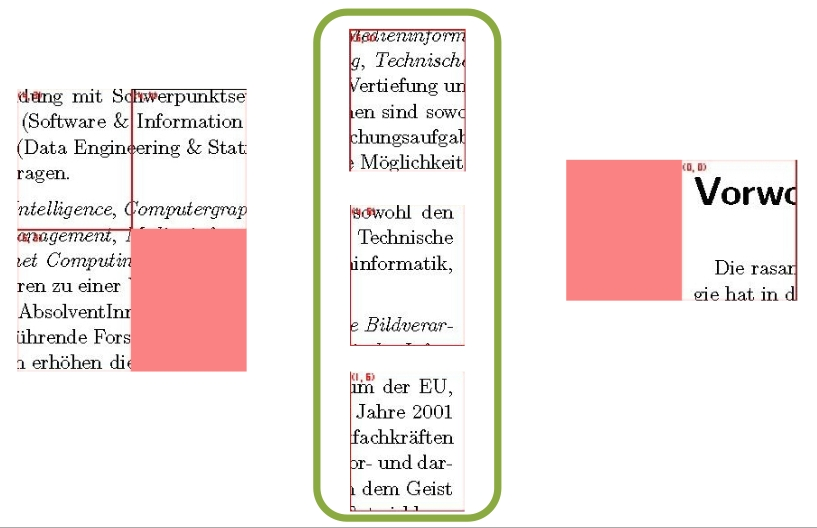
\includegraphics[width=\textwidth]{normPres1}
                \caption{Here we are trying to place one of the 3 shreds in the green rectangle into one of the two red slots. We want to identify the best of the 6 possible placements.\vspace{2\baselineskip}}
        \end{subfigure}
        ~ 
        \begin{subfigure}[b]{0.49\textwidth}
                \centering
                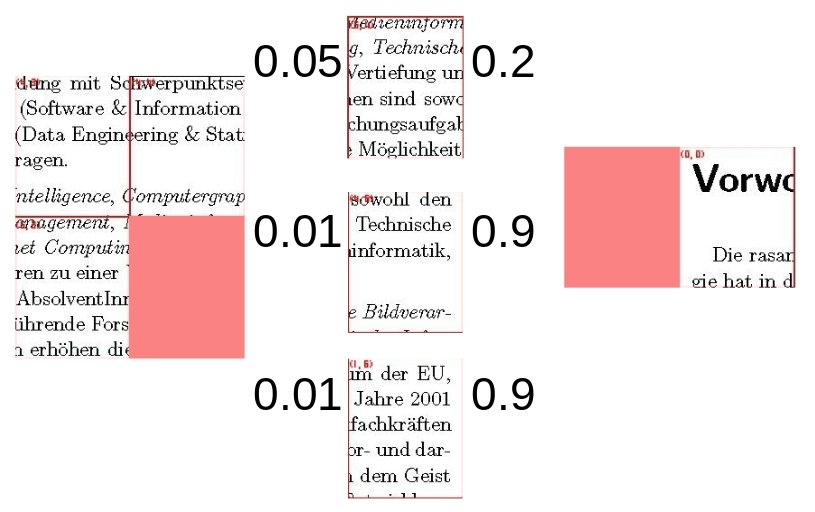
\includegraphics[width=\textwidth]{normPres2}
                \caption{The raw scores are shown. The scores for the left slot are lower since it has two neighbouring edges and therefore more probabilities to multiply together. For the right slot, two of the edges would give a ``white on white" match and therefore a very large score of 0.9.}
        \end{subfigure}
        ~ 
        \begin{subfigure}[b]{0.49\textwidth}
                \centering
                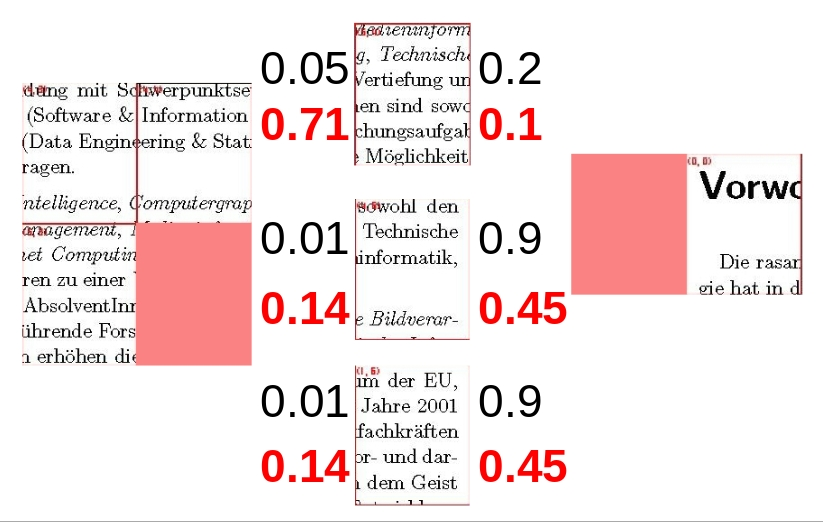
\includegraphics[width=\textwidth]{normPres3}
                \caption{Normalized scores shown in red. Number of pixels multiplied is irrelevant since the scores for each slot must sum up to 1. Probability mass for ``white on white" matches is split between the two possible matches, thus making it less likely that any of them will be picked.}
        \end{subfigure}
        ~ 
        \begin{subfigure}[b]{0.49\textwidth}
                \centering
                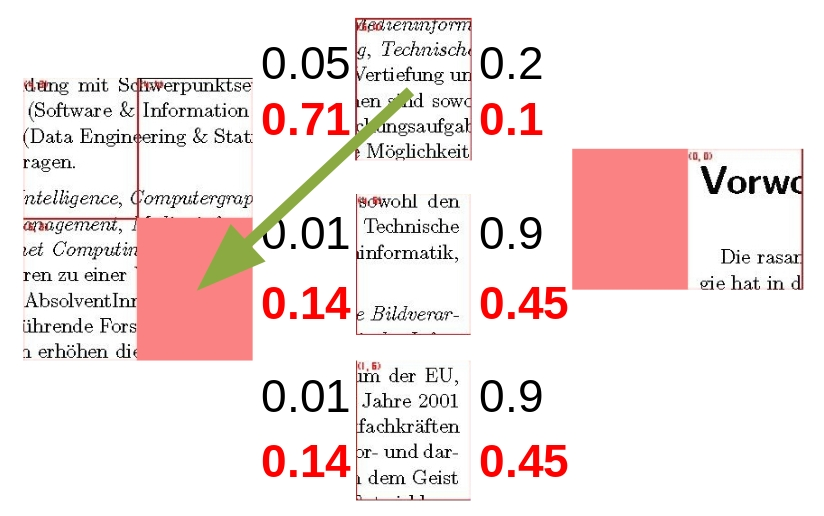
\includegraphics[width=\textwidth]{normPres4}
                \caption{The best placement is shown. Intuitively, this placement is best because its raw score is significantly larger than any of its competitor's. This score distribution means that this placement is the most likely to be correct.\vspace{1\baselineskip}}
        \end{subfigure}
        \caption{Properties of normalization. Both the issue with the varying number of pixels and the ``white on white" matches are solved by normalizing. In contrast, previous methods \cite{P1,P2} had to employ ad-hoc heuristics to address these problems.}
        \label{fig:norm}
\end{figure}
Additionally, as will be shown in Section \ref{chap4Eval}, the probabilistic score outperforms all previously formulated scoring functions.

Lastly, the effectiveness of probabilistic models, when applied to text data, has been repeatedly shown. Pixel prediction goes back to systems such as the 1981 JBIG lossless compression ISO standard (which tried to predict the value of a pixel using several features including 6 of its neighbours \cite{P3}) and is still employed in today's state of the art encoders \cite{P4}. 

\section{Description}

To the best of our knowledge, a probabilistic scoring function has never been previously used in this domain. We therefore choose to restrict ourselves to a relatively simple probabilistic model which can be used as a benchmark for future, more complex, approaches.

When looking at a proposed match, we try to estimate the probability that a candidate pixel is correct given several of its neighbouring pixels (called the candidate pixel's ``context", see Figure \ref{fig:probContext}). We refer to this conditional probability as \(\Pr( p \mid C(p,E_x) )\), where \(C(p,E_x)\) is the context of pixel $p$ when placed next to edge $E_x$. Ideally we'd want to learn these conditional probabilities by analysing the original document, which we obviously don't have access to. However, relatively few pixels are destroyed when shedding a document and we can assume that the ones that are destroyed are uniformly distributed over the space of contexts. Therefore the average distribution of pixels within the shreds will, in general, be a close approximation to the distribution of those in the original document. This similarity means that we can get a good estimate of the needed probabilities by obtaining the probabilities for each individual shred and then averaging them over all shreds.

\begin{figure}[h]
\centering

\includegraphics[width=0.8\textwidth]{context}
\caption{This shows a proposed match between the top 3 and the bottom 3 pixels. The model estimates the probability that the candidate pixel is white based on the four context pixels}
\label{fig:probContext}
\end{figure}

\clearpage
\subsection{Edge likelihood}

Once we obtain the conditional probabilities by analysing our shreds, then the raw probability of two edges matching can be calculated by sliding the context down the proposed edge and multiplying all the individual candidate pixel probabilities (see Figure \ref{fig:sliding}). 
\begin{figure}[h]
        \centering
        \begin{subfigure}[b]{0.49\textwidth}
                \centering
                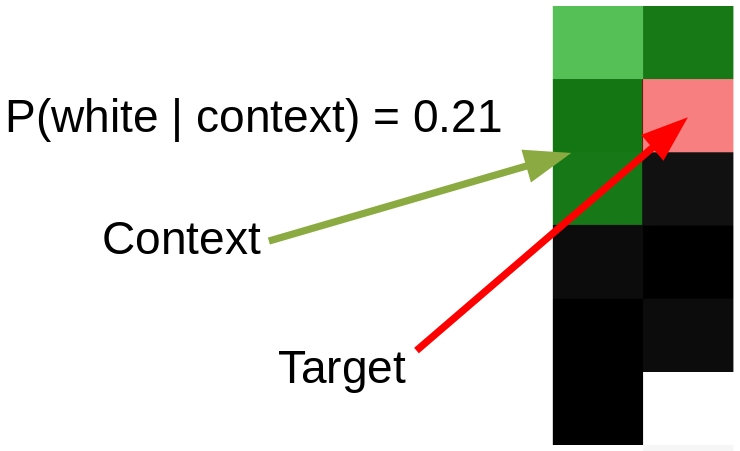
\includegraphics[width=\textwidth]{sliding1}
        \end{subfigure}
        ~ 
        \begin{subfigure}[b]{0.49\textwidth}
                \centering
                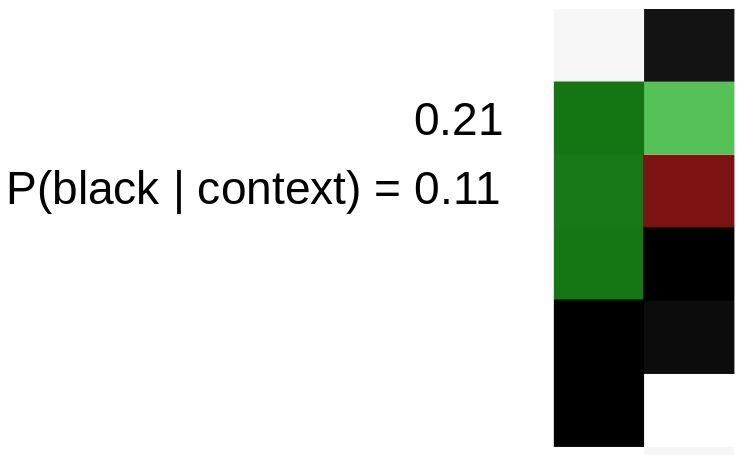
\includegraphics[width=\textwidth]{sliding2}
        \end{subfigure}
        ~ 
        \begin{subfigure}[b]{0.49\textwidth}
                \centering
                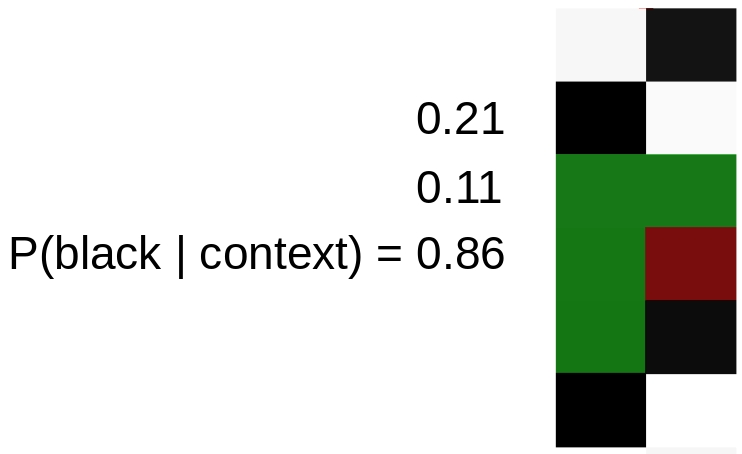
\includegraphics[width=\textwidth]{sliding3}
        \end{subfigure}
        ~ 
        \begin{subfigure}[b]{0.49\textwidth}
                \centering
                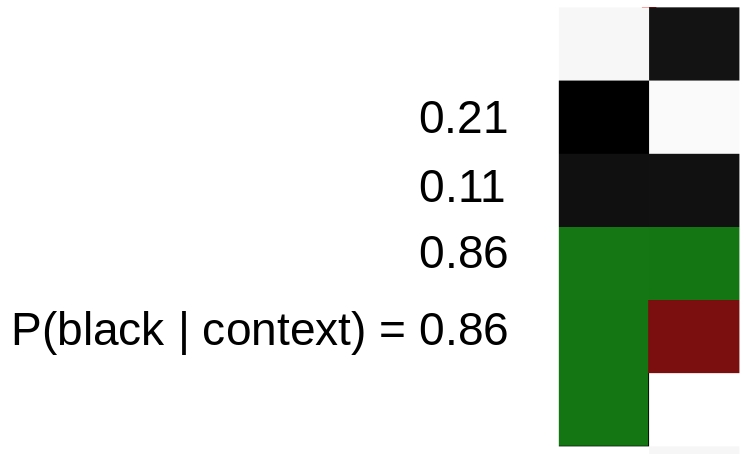
\includegraphics[width=\textwidth]{sliding4}
        \end{subfigure}
        ~
        \begin{subfigure}[b]{0.49\textwidth}
                \centering
                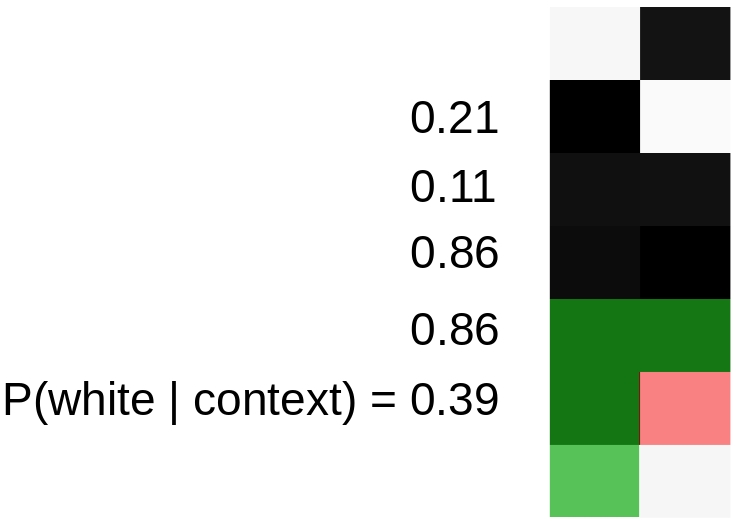
\includegraphics[width=\textwidth]{sliding5}
        \end{subfigure}
        ~ 
        \begin{subfigure}[b]{0.49\textwidth}
                \centering
                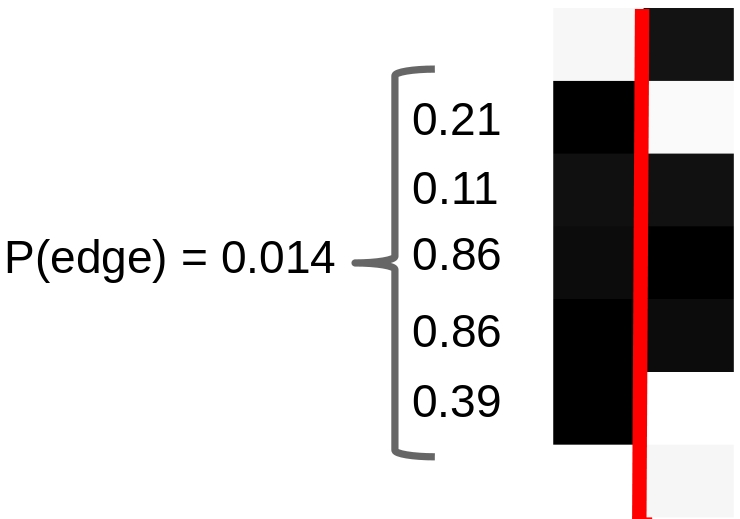
\includegraphics[width=\textwidth]{sliding6}
        \end{subfigure}
        \caption{The context slides down the proposed edge calculating a series of target pixel probabilities. All of these are then multiplied together to give the raw edge probability.}
        \label{fig:sliding}
\end{figure}

That is to say, if we have a proposed matching between edge \(E_1\) and edge \(E_2\), and \(E_1^x\) represents the $xth$ pixel on edge 1, then we would estimate the joint probability of the pixels in the two edges as being: \[\Pr(Pix(E_1),Pix(E_2)) = \prod_{i=1}^{len(E_2)} \Pr(E_2^i \mid C(E_2^i,E_1))\] A problem arises though, because the shape of the context prohibits us from taking the conditional probability for the first and last few pixels (depending on the length of the context). For these the best we can do is assign them the prior probability, \(\Pr(p)\), which is also extracted from the data simply by counting the proportion of white and black pixels. Therefore, when using the context of size 4 shown in Figure \ref{fig:probContext}, the edge probability will actually be: \[\Pr(Pix(E_1),Pix(E_2)) = \Pr(E_2^1) \Pr(E_2^{len(E_2)}) \prod_{i=2}^{len(E_2)-1} \Pr(E_2^i \mid C(E_2^i,E_1)) \]

\subsection{Normalization}\label{sect:norm}
The above, while being a good measure of the joint probability of pixels on an edge, is a function that will tend to decrease as $len(E_2)$ increases. The function will therefore tend to prefer shorter edges with less probabilities to multiply. Luckily, using probabilities gives us one more piece of information here. In the original file, every edge of every shred has only one correct match, since no two shreds are superimposed. Therefore, we know that the sum of the probabilities of all matches along one edge should sum up to one. In technical terms, if \(S_E\) is the set of all edges and \(Pr(E_1,E_2)\) is the probability that edges $E_1$ and $E_2$ match, then: \[\forall E_a \sum_{E_x \in S_E} \Pr(E_a,E_x) = 1 \] To obtain the edge probabilities that satisfy this constraint, the previous pixel probabilities are normalized along every edge. After the normalization, the preference for shorter edges is eliminated and the probabilities for different edges and pieces can be directly compared regardless of local features such as a particular edge length. Therefore, accounting for the normalization process, the final definition becomes\footnote{There actually is a further problem with the presented formula, namely that it doesn't account for edges belonging to the same piece. If \(E_1\) and \(E_2\) both belong to the same shred then obviously the probability that they match is 0 since a shred can't be in 2 places at once. This extra complication is ignored in the mathematical formalism for reasons of clarity}:  \[ \Pr(E_1,E_2) = \frac{\Pr(E_2^1) \Pr(E_2^{len(E_2)}) \prod_{i=2}^{len(E_2)-1} \Pr(E_2^i \mid C(E_2^i,E_1))}{\sum_{E_x \in S_E} \Pr(E_x^1) \Pr(E_x^{len(E_x)}) \prod_{i=2}^{len(E_x)-1} \Pr(E_x^i \mid C(E_x^i,E_1)) } \]


The normalization discussed above has an additional property, which ends up mitigating the predisposition towards whitespace that some of the other cost functions suffer from. The property in question is that if \(E_1\), \(E_2\) and \(E_3\) are very similar or identical edges then they will have less chance of being picked as the best match because the available probability mass of any match will be split equally among the 3 of them. Formally, if \(I_{E_x}\) is the set of edges identical to \(E_x\) then: \[\forall E_a \Pr(E_a,E_x) \leq \frac{1}{\mid I_{E_x} \mid}\] Since there are usually several white edges floating around in the edge set at any time, the above property ends up naturally discounting them without the need for any ad hoc heuristics (see Table \ref{tab:normalization} for a typical situation and Figure \ref{fig:sliding} for an additional illustration). To further discount the white on white matches we can introduce dummy white pieces into the shreds pool.

\begin{table}[h]
  \centering
  \begin{tabular}{|c|c|c|c|c|c|c|}
    \hline
    & \multicolumn{3}{|c|}{Raw probabilities} &  \multicolumn{3}{|c|}{Normalized probabilities} \\
    \cline{2-7}
    & Edge 3 & Edge 4 & Edge 5 & Edge 3 & Edge 4 & Edge 5 \\
    \hline
    Edge 1 & 0.90 & 0.90 & 0.20 & 0.45 & 0.45 & 0.10 \\
    \hline
    Edge 2 & 0.10 & 0.10 & 0.50 & 0.14 & 0.14 & 0.71 \\
    \hline
  \end{tabular}
  \caption{Here Edge 1, 3 and 4 are all white and as such have a very good raw score when matched together. After normalization however, the match between edge 2 and 5 is considered a better bet than any match containing edge 1, as edge 1's probability mass is distributed equally among the identical edges 3 and 4.}
  \label{tab:normalization}
\end{table}

\subsection{Learning}
Given the above descriptions, the problem of calculating the probability of any two edges matching can be reduced to the problem of estimating \(\Pr( p \mid C(p,E_x) )\) for an arbitrary pixel and its context. Depending on the size of the context, various machine learning methods could be used to accomplish this task. However, if the context is of the form shown in Figure \ref{fig:probContext}, then a simple exhaustive exploration of the context space becomes a possible solution. If the context is of size 4, as above, and we are working on black and white documents, then there are only \(2^4 = 16\) possible contexts. Since the number of contexts we can sample is directly proportional to the pixel count of the source image, for an average one page document, the number of observations will exceed 1 million. In practice this means that all 16 possible contexts are well represented in the document (a document where any of the contexts had less than 250 observations hasn't yet been encountered).

Of course the fit to the data will be limited by such a small context, however care must be taken when extending the context as it can easily lead to over-fitting. For instance using a context of size 7 instead of 4 usually leads to having several contexts with a number of observations in the single digits. Such values can, of course, not be trusted. Therefore it seems necessary to use more sophisticated methods in conjunction with a larger context. 

One such attempt was made by using neural networks. Different architectures were tried, with both contexts of size 4 and 7, however no significant difference was found when compared with the above direct estimation. It's likely that a context of 7 was still too small for the neural networks to manage to gain an advantage over direct estimation. Therefore the neural networks were abandoned as the longer training time could not be justified on the small contexts used in this method. If, however, we were to extend the score to use a significantly larger context or an altogether different and more complex probabilistic model, then more involved learning methods would likely prove essential. 

\section{Evaluation}
\label{chap4Eval}
The evaluation measures used here work by comparing the edges predicted by the algorithm to the real edges. In order to obtain the predicted edges, for every edge, we simply take the most likely pair edge. If \(PredMatch(E_a)\) is a function that returns \(E_a\)'s predicted match, then:
\[PredMatch(E_a) = \arg\max_{E_x} \Pr(E_a,E_x) \]

\subsection{Comparison with Gaussian cost functions}
In order to perform this comparison, a function \(CorrMatch(E_a)\) is defined, which returns the correct match for edge $E_a$. With this function we can define the \(score(E_a)\) function as:
\[
score(E_a) =
\left\{
	\begin{array}{ll}
		1  & \mbox{if } CorrMatch(E_a) = \arg\max_{E_x} \Pr(E_a,E_x) \\
		0 & \mbox{otherwise } 
	\end{array}
\right.
\]
However, there's a mistake here. The problem is that \(\arg\max_{E_x} \Pr(E_a,E_x)\) is not guaranteed to return a single element. What we really need to check for then is \( CorrMatch(E_a) \in \arg\max_{E_x} \Pr(E_a,E_x) \). 

This change allows for multiple maximum likelihood matches, but doesn't account for the increased probability that the correct edge is within the predicted set by chance. In the extreme case, if the probability score returned the same value for every edge, then this scoring function would judge any pairing as correct. The solution is to discount the score based on the size of the predicted set (which also makes intuitive sense, since when a search is actually performed, if there are multiple matches with the same probability, the search will simply have to pick one at random). The final score function is:
\[
score(E_a) =
\left\{
	\begin{array}{ll}
		\frac{1}{\mid \arg\max_{E_x} \Pr(E_a,E_x) \mid}  & \mbox{if } CorrMatch(E_a) \in \arg\max_{E_x} \Pr(E_a,E_x) \\
		0 & \mbox{otherwise } 
	\end{array}
\right. 
\]
Therefore the proportion of correctly predicted edges (where \(S_E\) is again the set of all edges) is:
\[
predictedCorrect = \frac{\sum_{E_x \in S_E} score(E_x)}{\mid\left\{E_a \mid CorrMatch(E_a) \in S_E\right\}\mid }
\]
Here the denominator is just counting the number of edges that actually have matches. This is necessary because using \(\mid S_E \mid \) instead would also count the outer edges which have no correct match.

Calculating analogous measures for the cost functions defined in \cite{P1} and \cite{P2} allows us to compare the three methods and shows the probabilistic score as having a relatively consistent advantage\footnote{In the presented graph, the advantage only manifests on samples with more than 50 shreds. The performance on the small cases is very volatile, causing the results of the methods to vary from document to document. The performance on the larger instances is, however, consistently in favour of ProbScore.} over the other functions (see Figure \ref{fig:costComp}).

\begin{figure}[h]
\centering
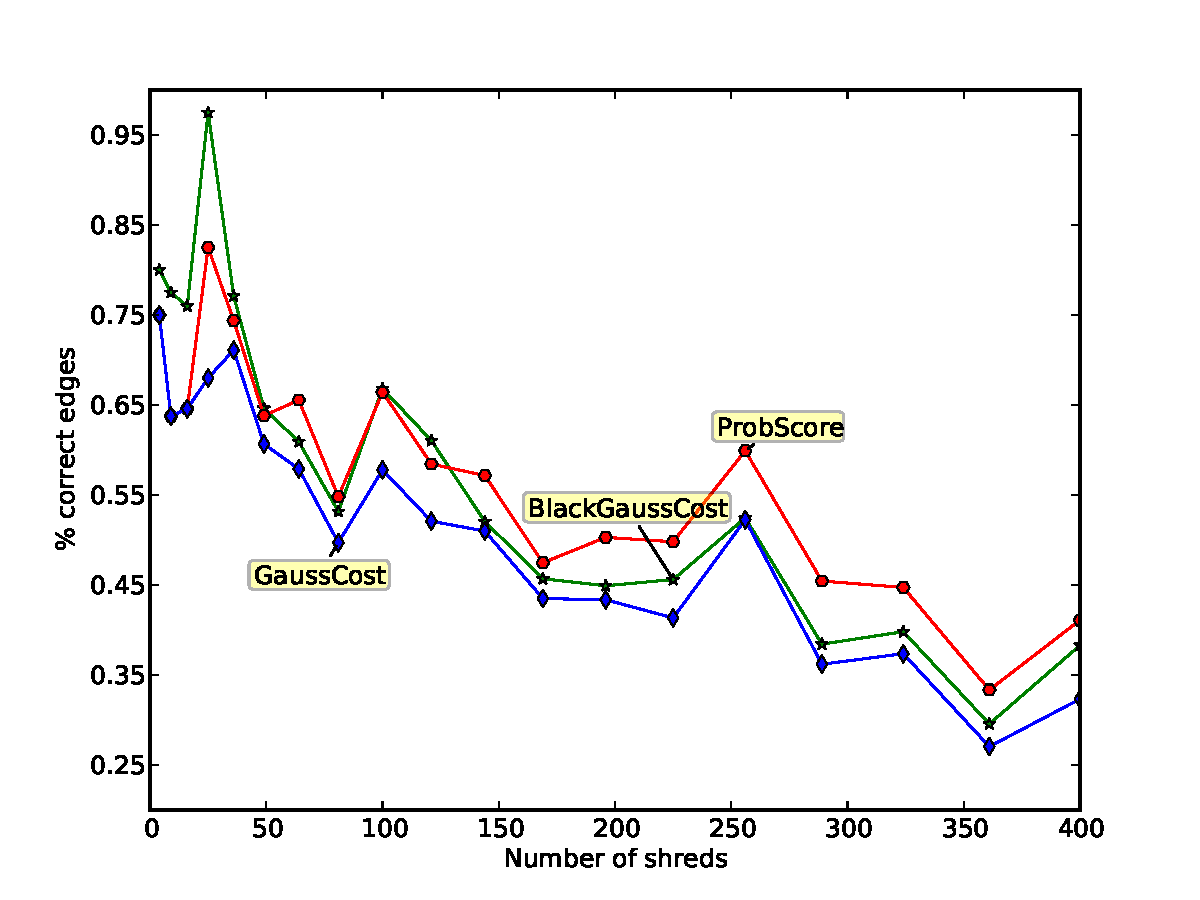
\includegraphics[width=\textwidth]{costComp}
\caption{The probabilistic score has better results on medium and large instances than the cost functions presented in \cite{P1} (GaussCost) and \cite{P2} (BlackGaussCost)}
\label{fig:costComp}
\end{figure}

\subsection{Validity of predicted probabilities}
As mentioned in the Motivation, there is another (perhaps more natural) evaluation that we can perform. Namely comparing the predicted and observed probabilities for our predicted edge matches. The observed probabilities are calculated exactly as in the previous section, and the predicted probabilities are recorded for every predicted match. 

The formula $bucket = \lfloor prob * 10 + 0.5\rfloor$ is used to place the predicted probabilities into one out of a total of 10 buckets. The observed and predicted probabilities are then averaged within each bucket, and the process is repeated for different number of shreds. The resulting graph is Figure \ref{fig:probComp}.
\begin{figure}[h]
\centering
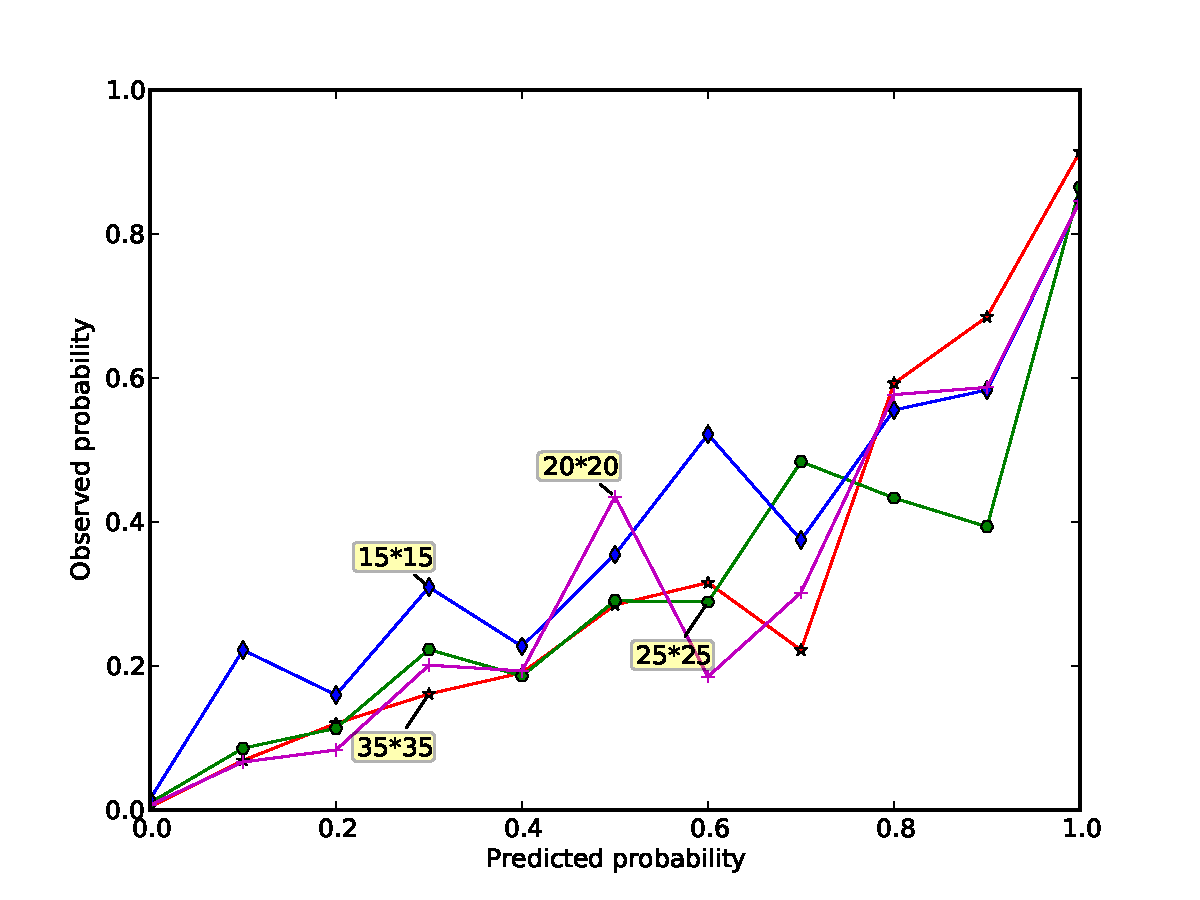
\includegraphics[width=\textwidth]{predObsProb}
\caption{The labels show the number of cross-cut shreds. As the number of shreds increases the relationship between the predicted and observed probability degrades. However the overall shape of the curve is still generally increasing, so a higher predicted probability will usually translate into a higher observed probability and for large predicted probabilities the method is quite accurate}
\label{fig:probComp}
\end{figure}

\subsection{Robustness}
\label{chap4Rob}
Another important aspect worth evaluating is the robustness of the method. When used in real life situations it is unlikely that documents will always be high-resolution, perfectly cut into shreds and completely smudge-free. In order to test this, the results obtained on an image are compared to those obtained when various types of noise are added to the image. 

The types of noise analysed are: downsampling, flipping random pixels and shuffling random pixels around their original position (see Figure \ref{fig:noiseTypes}). 

\begin{figure}[H]
        \centering
        \begin{subfigure}[b]{0.4\textwidth}
                \centering
                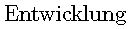
\includegraphics[width=\textwidth]{EntOrig}
                \caption{Original image}
        \end{subfigure}
        ~ 
        \begin{subfigure}[b]{0.4\textwidth}
                \centering
                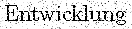
\includegraphics[width=\textwidth]{EntNoise}
                \caption{10\% of bits are randomly flipped}
        \end{subfigure}
        ~ 
        \begin{subfigure}[b]{0.4\textwidth}
                \centering
                
\includegraphics[width=\textwidth]{EntDown}
                \caption{The image is downsampled by a factor of 1.5}
        \end{subfigure}
        ~ 
        \begin{subfigure}[b]{0.4\textwidth}
                \centering
                
\includegraphics[width=\textwidth]{EntSpread}
                \caption{Pixels are randomly shuffled to one of their neighbours}
        \end{subfigure}
        \caption{How one word of the image is modified by the various types of noise}
        \label{fig:noiseTypes}
\end{figure}

The score evaluation is run on the original and modified documents, and the results are shown in Figure \ref{fig:robustness}. 

\begin{figure}[H]
\centering
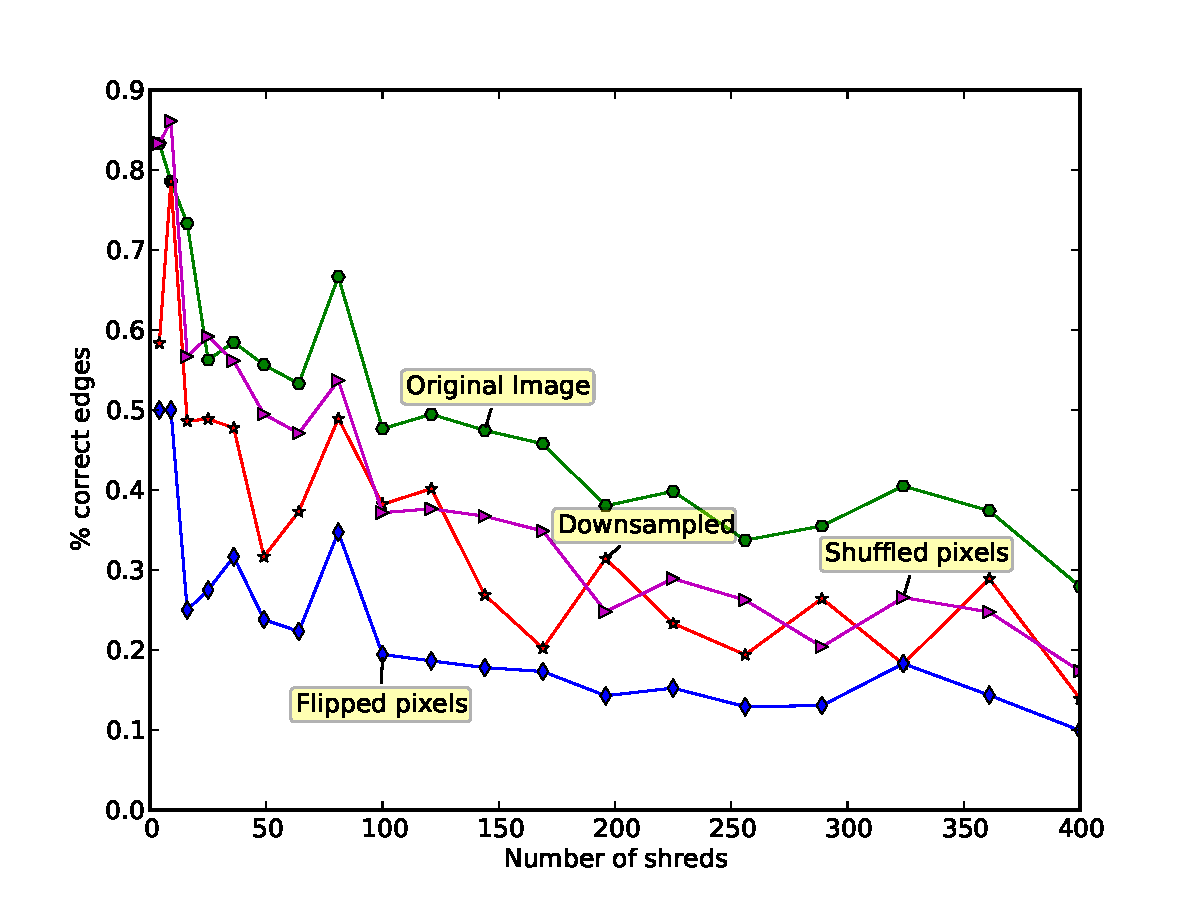
\includegraphics[width=\textwidth]{robustness}
\caption{Degradation of performance between original image and 3 noisy images}
\label{fig:robustness}
\end{figure}

Since the probabilistic scoring function is unique for each document, as it is trained on the noisy shreds, we'd like to see if this gives it an advantage when compared to the stationary Gaussian. Therefore, the probabilistic scoring function is compared with the best Gaussian alternative on all types of noise in Figure \ref{fig:robComp}. As expected some performance degradation is observed in all cases. It is interesting to note that the largest reduction in performance is caused by the random pixel flipping. This can be explained by the fact that the other types of noise are restricted by the existing structure of the document, if you have a section of white pixels, neither downsampling nor shuffling can introduce a black pixel into it. The algorithm seems to suffer more from the unrestrained randomness exhibited by the flipping. The good news is that in real life scenarios most noise should not be completely random and we'd expect it to be more similar to the downsampling and shuffling types of noise than to the pixel flipping.

\begin{figure}[h]
        \centering
        \begin{subfigure}[b]{0.49\textwidth}
                \centering
                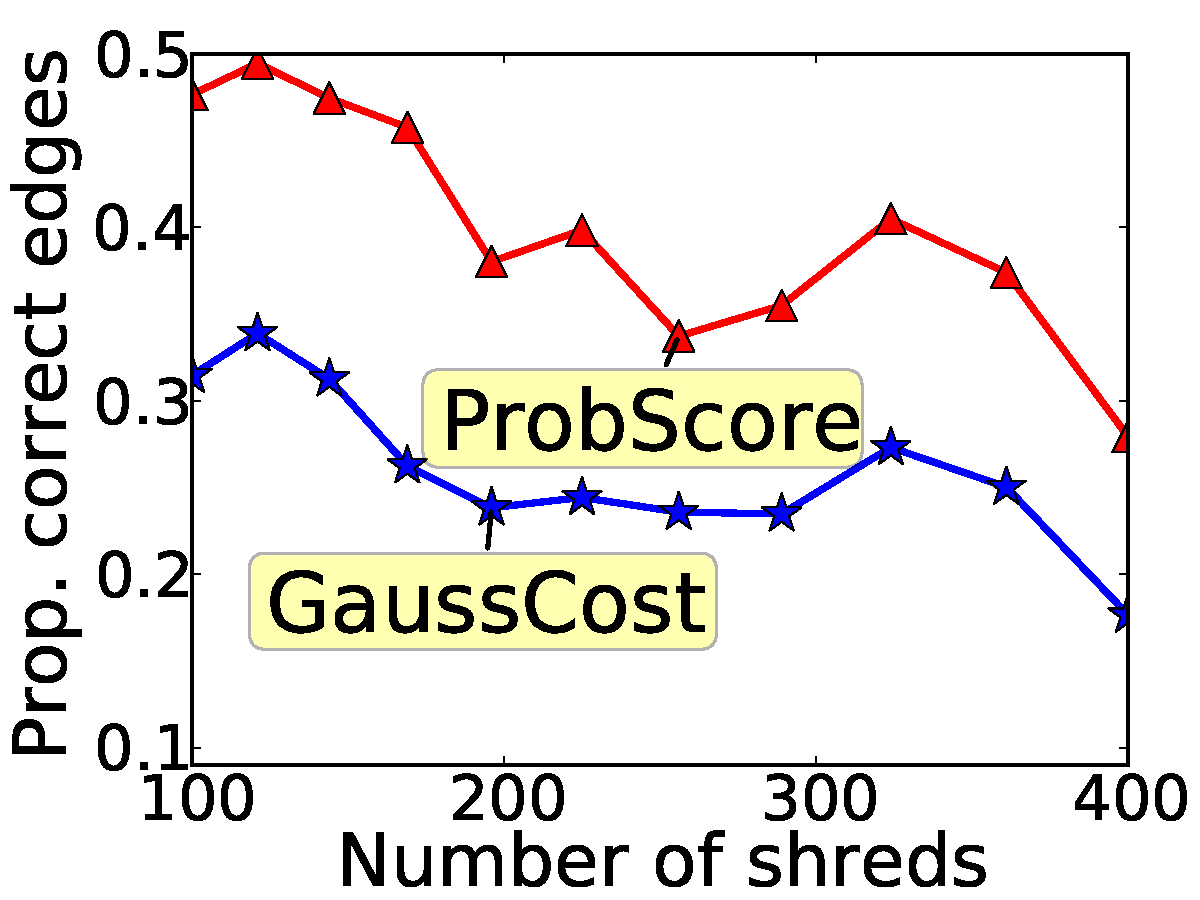
\includegraphics[width=\textwidth]{origComp.pdf}
                \caption{Original image}
        \end{subfigure}
        ~ 
        \begin{subfigure}[b]{0.49\textwidth}
                \centering
                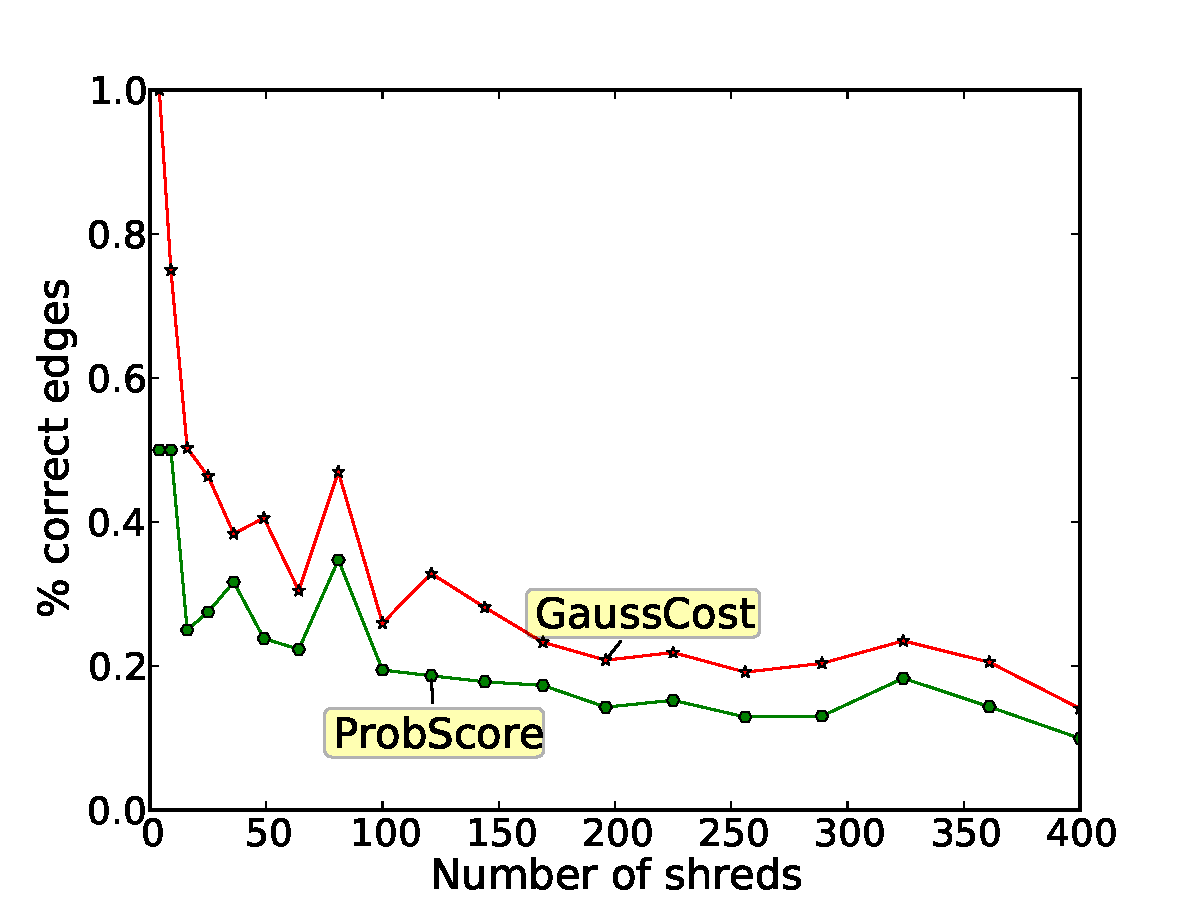
\includegraphics[width=\textwidth]{noise.pdf}
                \caption{10\% of bits are randomly flipped}
        \end{subfigure}
        ~ 
        \begin{subfigure}[b]{0.49\textwidth}
                \centering
                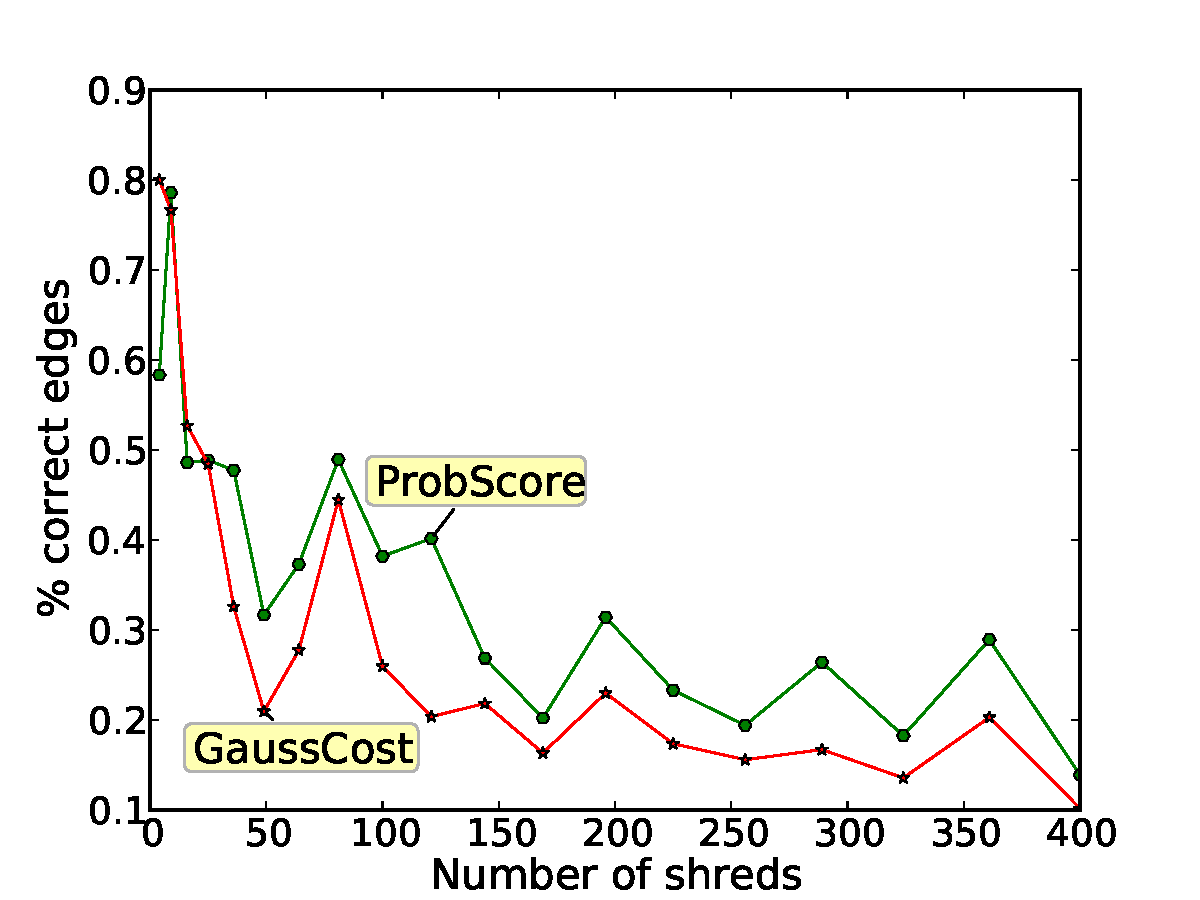
\includegraphics[width=\textwidth]{downsample.pdf}
                \caption{The image is downsampled by a factor of 1.5}
        \end{subfigure}
        ~ 
        \begin{subfigure}[b]{0.49\textwidth}
                \centering
                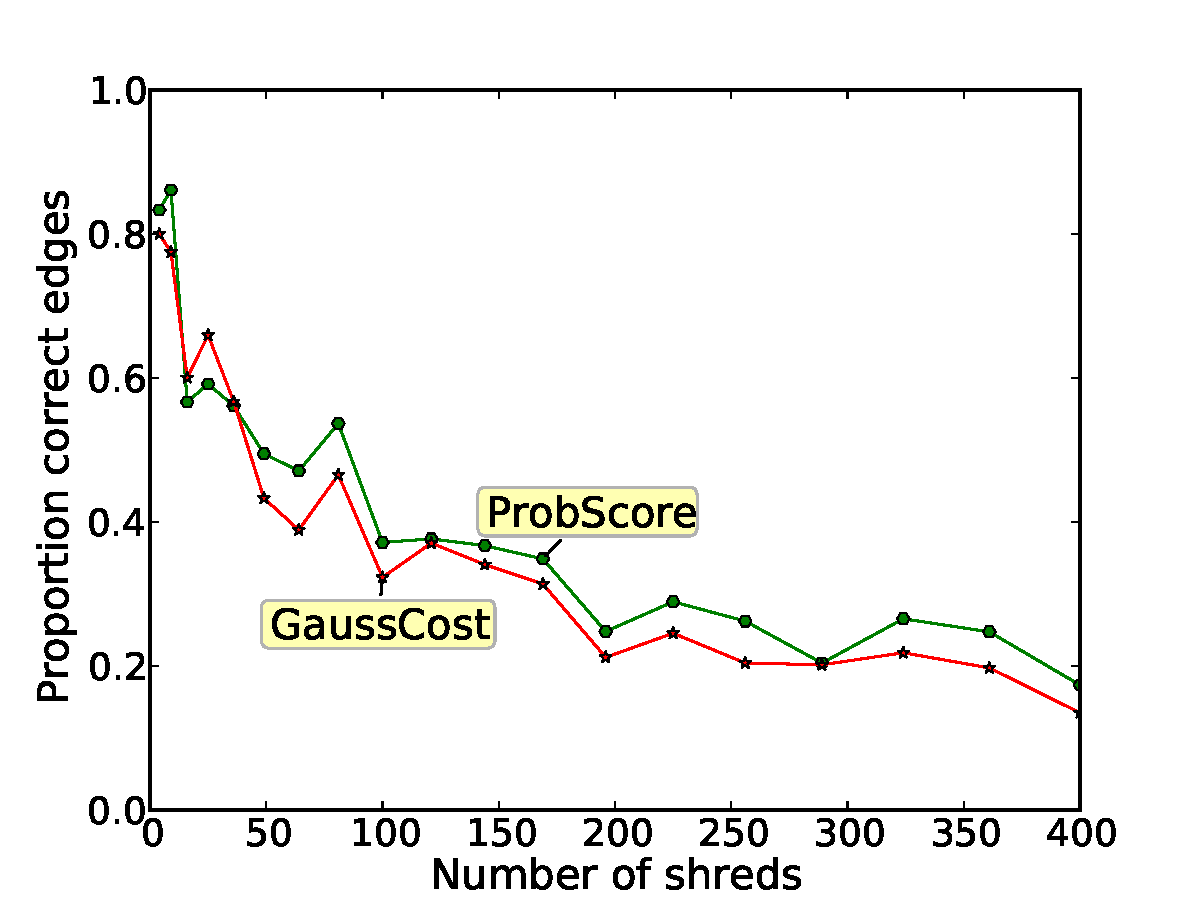
\includegraphics[width=\textwidth]{shuffle.pdf}
                \caption{Pixels are randomly shuffled to one of their neighbours}
        \end{subfigure}
        \caption{ProbScore outperforms the best Gaussian cost function on 3 out of 4 noise variants. The poor performance on case (b) is due to the simple probabilistic model not being able to cope well with completely random noise. However, this type of noise is less likely to be encountered than the other variants.}
        \label{fig:robComp}
\end{figure}

\section{Drawbacks}

Finally, we'll look at some of the flaws in the probabilistic scoring function and at some possible solutions.

\subsection{Uniformity assumption}
Learning a single set of conditional values of the form \(\Pr(p_i \mid C(p_i,E_x)) \), where the number of possible contexts $C(p_i,E_x)$ is small, implicitly makes the assumption that these conditional values are relatively uniform over the whole document. This is usually a reasonable assumption to make if the documents we're interested in are all text. However this assumption is certainly not always justified. Consider the document from Figure \ref{fig:tableText}. Here we can clearly see that there are two distinct regions, the text region and the table region. An algorithm which tries to fit a single valued model with a small context to this document cannot achieve very good results, because this document cannot be described well by such a model. The problem will only be compounded if we're looking at multiple shredded pages from possibly different documents.

\begin{figure}[h]
\centering
\includegraphics[width=10cm]{tableText}
\caption{A document in which the uniformity assumption is wrong.}
\label{fig:tableText}
\end{figure}

One solution here is to make the context complex enough to remove the uniformity assumption, by being able to tell between the different regions in the document. This could be done by using a significantly larger context size, or perhaps by using a different probabilistic model that takes higher level features into account (see also Section \ref{chap5NE}). A different approach would be to first split the shreds into categories and then learn a set of conditioned probabilities for every category. In theory this could also help reduce the problem size, by separating the documents into smaller uniform regions. However, avoiding overfitting might be difficult in this scenario. For instance, we wouldn't want the model to decide that every boldfaced piece of text belongs together in a separate uniform region.

\subsection{Lack of symmetry}
If \(E_x\) and \(E_y\) are two edges and \(E_x^{rot}\) and \(E_y^{rot}\) are the previous edges rotated by \(180^\circ\) then we might reasonably expect that \[\forall E_x \forall E_y \Pr(E_x,E_y) = \Pr(E_y^{rot},E_x^{rot})\] This would be a good property to have, since we are essentially comparing the exact same edge matching in both situations. However, the current probabilistic model offers no such guarantee. In particular the probabilistic model cannot guarantee that \(P(E_x,E_y) = P(E_y^{rot},E_x^{rot}) \) because it is not assured (and indeed quite unlikely) that enough data was present for these two conditional probabilities to have converged to the same value.

Depending on the situation this deficiency could be ignored. It is possible, however, that the search function being employed will assume the score to be symmetric. In that case, the best solution seems to be to calculate both \(\Pr(E_x,E_y)\) and  \(\Pr(E_y^{rot},E_x^{rot})\) and re-assign both probabilities to some number in between the 2 original probabilities (arguments could be made for either $min$, $max$ or $avg$). Care should be taken that this re-assignment is done before the normalization step, otherwise the values will no longer add up to 1.

\subsection{Ignoring non-edge information}
\label{chap5NE}
This problem is common to both the probabilistic score and all the cost functions presented above. It is also the hardest to fix. Figure \ref{fig:fakeMatch} shows an error made on a 5x5 cross-cut document. It is interesting to notice how even in a document cut into only 25 pieces such a convincing false match can occur. As the size of the shreds and therefore the amount of information available to our scoring function decreases further we can expect a huge number of such mistakes, making reconstruction of any non-trivial cross-cut document problematic.

\begin{figure}[h]
\centering
\includegraphics[width=0.6\textwidth]{conf.jpg}
\caption{An incorrect match that would be very difficult to detect by a cost/score function which only looks at the edge pixels}
\label{fig:fakeMatch}
\end{figure}

The solution here likely involves combining multiple scoring functions looking at different sets of features, both higher and lower level. Luckily, as mentioned above, the probabilistic score can easily accommodate any such scoring functions as long as they can express their result as a probability. One possible higher level scoring functions is discussed in Section \ref{chap4Mod}.

\section{Modularity}
\label{chap4Mod}

One of the big advantages of using a probabilistic scoring function is that this allows for very easy composition with any other probabilistic function. As a proof-of-concept implementation, we propose a very simple function, called ``RowScore", and show how it can be composed with the probabilistic scoring function.

``RowScore" is based on the idea that rows in neighbouring shreds should generally match. We identify all the rows in the shreds and, when looking at a potential shred match, sum up all the discrepancies between neighbouring rows. In order to formally define this sum, we specify a function $neighRow$ such that, if $A$ is a shred and $t$ is a y coordinate, then: \[neighRow(A,t) = \mbox{the y coordinate of the row in A closest to location t} \] If we also define $rows(A)$ to be a set of the y coordinates of all rows in shred $A$, the measure of how well shreds $A$ and $B$ match is then given by: \[RowDist(A,B) = \sum_{t \in rows(A)} |t - neighRow(B,t)| \] In order to translate this distance into a probability, we can make a simple Gaussian assumption. We want to assign the most probability mass to the case when the distance is $0$, so this is the mean of the distribution. Therefore the final form of ``RowScore" is\footnote{The variance of the normal distribution can be set empirically, but should take account of the size of the shreds. In experiments we have seen that the performance is not very sensitive to this value.}: \[ RowScore(A,B) = \frac{\displaystyle {e}^{-\frac{x^2}{2\sigma^2}}}{\sigma \sqrt{2\pi}} \]

Using the above method, we can give the probabilistic scoring function a small but consistent boost in performance, as shown in Figure \ref{fig:rowScore}.
\begin{figure}[h]
\centering
\includegraphics[width=0.95\textwidth]{rowScore.pdf}
\caption{Even the extremely simple ``RowScore" model gives a noticeable and consistent boost in performance to the probabilistic scoring function.}
\label{fig:rowScore}
\end{figure}

\addtocontents{toc}{\newpage}
\chapter{Heuristic Search}
\label{chap5}
\section{Motivation}
As discussed in the Chapter \ref{chap3}, many complex methods have been applied to the search problem. These methods take varied approaches such as reduction to a travelling salesman problem and making use of industrial solvers \cite{P1}, variable neighbourhood search \cite{P1,P5,P7}, genetic algorithms \cite{P7,P19}, ant colony optimization \cite{P5,P19} and reformulation as an integer linear programming problem \cite{P6}.

However, at least in the first instance, we decide to focus upon relatively simple greedy heuristics. Some reasons for this decision are:
\begin{itemize}
\item The heuristics run significantly faster than the aforementioned methods. This allows for ease of prototyping and the ability to easily experiment with many variations on both the search and cost functions.
\item The inner-workings of the heuristics are transparent. This transparency allows for ease in diagnosing problems with either the heuristics themselves or with the cost functions. The transparency also allows for easy visualisation of every individual search step which enables us to observe exactly how errors occur and are how they are propagated. In contrast, using some of the previous methods would make it difficult to diagnose, for instance, whether an error is caused by the search or the cost function.
\item Any advanced search methods need to be compared against a solid baseline. These heuristics provide such a baseline.
\item Surprisingly good performance has been obtained using greedy heuristics. For instance, \cite{P2} reports that their simple heuristic search managed to outperform both a variable neighbourhood search and an ant colony optimization method.
\item The heuristics can cope with inputs containing missing shreds or extra shreds coming from different documents. This robustness is a consequence of the heuristic's bottom up formulation, which needs to make fewer assumptions than the top down optimizing solutions.
\end{itemize}

\section{Description}
\label{chap5Desc}
Despite the fact that most of the previous work has focused on complex search algorithms, a few greedy heuristics have been explored before. We first re-implement 3 of these heuristics which, in growing order of complexity, are: the \emph{Row building} heuristic \cite{P5}, the \emph{Prim based} heuristic \cite{P5} and the \emph{ReconstructShreds} heuristic \cite{P2}. More details about these techniques are available in Section \ref{chap2Search}. Additionally, we implement a fourth, novel, heuristic which is an extension of the ReconstructShreds version. 

The central idea behind the ReconstructShreds heuristic is that, at each search step, the best available edge should be added to the partial solution. A few steps of the execution of this algorithm are examined in Figure \ref{fig:kruskal}, where all groups of shreds of size 2 or larger are shown (i.e. the individual pieces, which are groups of size 1, are omitted from the figure). The algorithm will continue to add the best possible edge to the partial solution and thus enlarge and merge clusters until only 1 cluster is left. This final cluster is the algorithm's final solution. 

\begin{figure}[h]
        \centering
        \begin{subfigure}[b]{0.49\textwidth}
                \centering
                \includegraphics[width=\textwidth, height=4.5cm]{kruskal1}
                \caption{There are 3 clusters: A, B and C \vspace{2\baselineskip}.}
        \end{subfigure}
        ~ 
        \begin{subfigure}[b]{0.49\textwidth}
                \centering
                \includegraphics[width=\textwidth, height=4.5cm]{kruskal2}
                \caption{Best edge was between 2 shreds which belonged to neither cluster. Therefore a new cluster is created.}
        \end{subfigure}
        ~ 
        \begin{subfigure}[b]{0.49\textwidth}
                \centering
                \includegraphics[width=\textwidth, height=4.5cm]{kruskal3}
                \caption{Best edge was between a shred belonging to cluster B and one belonging to neither cluster. Therefore cluster B is enlarged.}
        \end{subfigure}
        ~ 
        \begin{subfigure}[b]{0.49\textwidth}
                \centering
                \includegraphics[width=\textwidth, height=4.5cm]{kruskal4}
                \caption{Best edge was between a shred belonging to cluster B and one belonging to cluster C. Therefore the two clusters are merged.}
        \end{subfigure}
        \caption{Four steps from the middle of a ReconstructShreds search are shown. The clusters are called A, B, C and D, the green pieces highlight the changes that occur in every step and the red pieces show the positions that are considered for the insertion of new shreds.}
        \label{fig:kruskal}
\end{figure}

\subsection{Analysis of ReconstructShreds}
This algorithm calculates all the edge probabilities and goes through the list in descending order. Whenever it encounters a valid edge, it adds it to the solution set (see Algorithm \ref{alg:RS} for the pseudocode \footnote{The pseudocode in this chapter assumes the existence of a disjoint-set data structure which can perform operations such as $InitSet(x)$ (create a set with the element $x$ in it), $GetSet(x)$ (return the set to which $x$ belongs) and various set operations such as $Union(S_x,S_y)$ and $Intersect(S_x,S_y)$}).

\begin{algorithm}[h]
\caption{The ReconstructShreds heuristic}
\begin{algorithmic}[1]
\Statex \Comment{Takes the set of edges and the set of shreds as input} 
\Procedure {ReconstructShreds}{$S_{edges}$, $S_{shreds}$} 
  \State $probs \gets []$ \Comment{Initialize 2 empty arrays for the probabilities and edges}
  \State $edges \gets []$ 
  \ForAll{$E_x \in S_{edges}$} 
    \ForAll {$E_y \in S_{edges}$}
      \State $probs[(E_x,E_y)] \gets \Pr(E_x,E_y)$ \Comment{Calculate and store all the probabilities}
    \EndFor
  \EndFor
  \Statex
  \State $setsLeft \gets |S_{shreds}|$  \Comment{Initially every shred is its own set, initialize these}
  \ForAll{$S_x \in S_{shreds}$}
    \State $InitSet(S_x)$
  \EndFor
  \Statex
  \While{$setsLeft > 1$} \Comment{Get the edges with the max probability}
    \State $(E_x,E_y) \gets \arg\max_{(E_x,E_y)} probs[(E_x,E_y)]$ 
    \State $S_x \gets GetSet(E_x)$ \Comment{Retrieve the sets of these 2 edges} 
    \State $S_y \gets GetSet(E_y)$
    \If{$S_x \neq S_y ~ \& ~ mergePossible(E_x,E_y)$} 
      \State $S_x \gets Union(S_x,S_y)$ \Comment{If the edge is valid, merge the two sets}
      \State $S_y \gets Union(S_x,S_y)$
      \State $edges.append((E_x,E_y))$
      \State $setsLeft \gets setsLeft - 1$  
    \EndIf
    \State $probs[(E_x,E_y)] \gets 0$ \Comment{make sure the processed edge isn't picked again} 
  \EndWhile
  \Statex
  \State \textbf{return} $edges$ \Comment{The set of returned edges describes a complete solution} 
\EndProcedure
\end{algorithmic}
\label{alg:RS}
\end{algorithm}

The problem with this approach is that the probabilities used are static and therefore the algorithm is completely ignorant of the formed partial solution. Its only interaction with the current state of the solution occurs via the $mergePossible(E_x,E_y)$ function which just tells the algorithm if the current solution allows for that particular merge. In particular, the algorithm takes no account of the fact that when merging 2 sets of pieces, several new edges may form. Therefore the ReconstructShreds heuristic would be happy to merge two large sets of pieces based on 1 good edge resulting from the merge even if several other terrible edges also result from that same match (see Figure \ref{fig:rsp}).

\begin{figure}[h]
    \centering
    \includegraphics[width=\textwidth]{recShredProb}
    \caption{Here two potential matches for the red slot are shown. The first match is a single white piece, while the second match is a group of 3 shreds that perfectly aligns with our target shreds. Since ReconstructShreds will only look at one edge, both matches will have an identical score, namely that assigned to all white on white matches. ReconstructShreds cannot take advantage of the extra information gained since the second white shred was merged with additional shreds.}
    \label{fig:rsp}
\end{figure}

Our algorithm is designed to address this shortcoming.

\subsection[Kruskal based heuristic] {Kruskal based heuristic\footnote{This method is called a \emph{Kruskal based heuristic} because the main goal of the method, namely that of always adding the best available edge to the solution, is analogous to the goal of the minimum spanning tree algorithm, Kruskal \cite{P9}. Therefore the general Kruskal method can be extended to this specific problem, with the only additional difficulty of having to reject potential matches which would result in 2 shreds overlapping. Indeed ReconstructShreds is already an extension of the Kruskal method, though the authors of \cite{P2} do not identify it as such}} 
Our approach towards resolving the problem observed in ReconstructShreds is to recalculate the probabilities of two edges matching at every iteration. By doing so we can take into account all the additional matches that would result when the sets corresponding to the 2 edges are merged (see Algorithm \ref{alg:kruskal}). 

\begin{algorithm}[h]
\caption{The Kruskal based heuristic}
\begin{algorithmic}[1]
\Procedure {Kruskal}{$S_{edges}$, $S_{shreds}$} 
  \State $edges \gets []$ 
  \State $setsLeft \gets |S_{shreds}|$ 
  \ForAll{$S_x \in S_{shreds}$}
    \State $InitSet(S_x)$
  \EndFor
  \Statex
  \While{$setsLeft > 1$}
    \State $probs \gets []$ \Comment{Probability calculation is done for every iteration}
    \ForAll{$E_x \in S_{edges}$} 
      \ForAll {$E_y \in S_{edges}$}
        \State $probs[(E_x,E_y)] \gets getProb(E_x,E_y)$  \Comment{Helper function is called}
      \EndFor
      \State $normalize(probs, E_x, S_{edges})$ \Comment{An extra normalization step is needed}
    \EndFor
    \State $(E_x,E_y) \gets \arg\max_{(E_x,E_y)} probs[(E_x,E_y)]$
    \State $S_x \gets GetSet(E_x)$ 
    \State $S_y \gets GetSet(E_y)$
    \If{$S_x \neq S_y ~ \& ~ mergePossible(E_x,E_y)$} 
      \State $S_x \gets Union(S_x,S_y)$ 
      \State $S_y \gets Union(S_x,S_y)$
      \State $edges.append((E_x,E_y))$
      \State $setsLeft \gets setsLeft - 1$  
    \EndIf
    \State $probs[(E_x,E_y)] \gets 0$ 
  \EndWhile
  \Statex
  \State \textbf{return} $edges$ 
\EndProcedure
\end{algorithmic}
\label{alg:kruskal}
\end{algorithm}

The differences between the Kruskal and the ReconstructShreds algorithms are:
\begin{itemize}
\item The probability calculation has been moved inside the \emph{while loop}, and thus our calculated probabilities need not be static any more.
\item Rather than simply taking the pre-calculated probability $\Pr(E_x,E_y)$ as the final measure of the likelihood of a match between $E_x$ and $E_y$, the helper function $getProb(E_x,E_y)$ is now called instead. This new function checks the proposed merge and identifies all the new edges that would be formed if this merge is selected (for convenience we assume the set of edges $S_x$ has a function $S_x.neighbours()$ which returns all the pairs of edges that are neighbours under this merge). The final probability is then given by multiplying the individual probabilities for every newly created edge (see Algorithm \ref{alg:getProb}).

\begin{algorithm}[h]
\caption{The getProb helper function}
\begin{algorithmic}[1]
\Procedure {getProb}{$E_x$, $E_y$}
  \State $prob \gets 1.0$
  \State $S_x \gets GetSet(E_x)$ 
  \State $S_y \gets GetSet(E_y)$ \Comment{Get the set of the proposed match}
  \State $merged \gets Union(S_x,S_y)$ 
  \ForAll{$E_a \in S_x$} \Comment{Multiply probs of new neighbours created by the match}
    \ForAll {$E_b \in S_y$}
      \If{$ (E_a,E_b) \in merged.neighbours()$} 
      \State $prob \gets prob * \Pr(E_a,E_b)$
      \ElsIf{$ (E_b,E_a) \in merged.neighbours()$}
      \State $prob \gets prob * \Pr(E_b,E_a)$
      \EndIf
    \EndFor
  \EndFor
  \State \textbf{return} $prob$
\EndProcedure
\end{algorithmic}
\label{alg:getProb}
\end{algorithm}

\item A normalization step is added. This is necessary because, by potentially multiplying the probabilities of several edges together to get the probability of our match, the sum of all probabilities is no longer guaranteed to be 1. Formally, after the normalization step taken in the calculation of the $\Pr(E_x,E_y)$ values (see Section \ref{sect:norm}) we had the following assurance: \[\forall E_a \sum_{E_x \in S_E} \Pr(E_a,E_x) = 1 \] We would like to have the same assurance regarding $getProb(E_x,E_y)$, which is why the additional normalization step is required. As before, the normalization step takes the form: \[ normProb(E_x,E_y) = \frac{getProb(E_x,E_y)}{\sum_{E_a \in S_E} getProb(E_x,E_a)} \]
\end{itemize}


\subsection{Evaluating the heuristics}
\label{chap5Eval}
We turn to evaluating the strengths and weaknesses of the algorithms discussed above.\footnote{RBH and Prim are reviewed in Section \ref{chap2Search}.} Towards this purpose we run two sets of tests. 

Firstly, we look at the performance offered by the various search functions. This is accomplished by running all the heuristics on the same input document, using the same cost function and then comparing the number of correct edges observed in the output (see Figure \ref{fig:searchScore}). 
\begin{figure}[h]
  \centering
  \includegraphics[width=\textwidth]{searchScores.pdf}
  \caption{The proportion of correct edges found by each search heuristic as the number of shreds increases.}
  \label{fig:searchScore}
\end{figure}
These results show that the Row Building Heuristic performs significantly worse than the others, but the performance of the top 3 heuristics is somewhat hard to compare. 

In order to try to improve upon this, a new evaluation method is proposed. This method tries to evaluate how hard it would be for a human to understand what is printed on the returned document. We therefore look at the number of moves a human would have to make to obtain the correct solution from a solution received from one of the heuristics. This assumes that the human can spot all areas of the document that are correctly reconstructed, extracts these areas and places them correctly relative to one another. Using this new evaluation method, we get Figure \ref{fig:searchGroups}, which shows that Kruskal is usually the best performing heuristic, even if not by a large margin.

\begin{figure}[h]
  \centering
  \includegraphics[width=\textwidth]{searchGroups.pdf}
  \caption{The number of moves left to perform to reach a correct solution, after running the search heuristics.}
  \label{fig:searchGroups}
\end{figure}

Secondly, we analyse the scalability of the algorithms. In real world scenarios an unshredder would potentially have to work with thousands, or even tens of thousands of pieces, which makes scalability an important factor to consider. For comparison purposes, the runtime of several more complex search functions are also shown in Figure \ref{fig:searchTime}. 
\begin{figure}[h]
  \centering
  \includegraphics[width=\textwidth]{searchTime.pdf}
  \caption{Runtime comparison for 3 of the heuristics and several previously reported methods taken from \cite{P2,P5,P7}. ``ACO" is Ant Colony Optimization and ``$HV^2$" and ``$BV^2$" are two different genetic algorithms. }
  \label{fig:searchTime}
\end{figure}

As can be seen. even though the heuristics were not implemented with speed in mind\footnote{The heuristics are written in python, while the quoted optimization methods are written in C. Additionally, the implementation of ``Kruskal" is a proof-of-concept and has not been optimized at all. A non-naive reimplementation could bring its performance more in line to that of ``Prim".}, they are significantly faster than the top-down optimization methods.

\section{Cascading}
\label{chap5Casc}
All of the greedy methods presented thus far have in common an inability to correct errors. This makes them prone to a cascading effect through which an error made early in the search process can have a major effect on the result. Since there is no means through which to move the wrongly placed shred, the search will instead try to find additional pieces which match well with said shred, and these pieces will have a significant probability of also being wrong. 

In order to quantify the magnitude of this issue it is helpful to plot the function: $Error_{search}(x)$, where $x = Error_{cost}$. This function shows the proportion of errors that the search function commits when given a score function with a certain error rate. The results of this experiment\footnote{This experiment was run on synthetic data. We simulated a score function with a fixed error rate and gave the output of this function to the search heuristics} (see Figure \ref{fig:cascading}) are telling.

\begin{figure}[h]
  \centering
  \includegraphics[width=\textwidth]{cascading.pdf}
  \caption{The effect the error in cost/score has on the final error of the method for both search heuristics on 5*5 shreds and for Prim on 30*30 shreds }
  \label{fig:cascading}
\end{figure}

Even on a tiny 5 by 5 instance, in order for the Prim heuristic to achieve 80\% accuracy the scoring function must be 95\% accurate. As can be seen, the problem only gets worse as the number of shreds increases. On a 30 by 30 instance Prim requires the same 95\% cost function accuracy rate in order to achieve a final accuracy of only 50\%.

In order to address this problem, several error correcting mechanisms were analysed. 

\newpage
\subsection{Making all shreds movable}
The simplest approach is to consider pieces that have already been placed as movable and treat them the same as the pieces which haven't been placed. Estimating the results of this formulation with the above cascading experiment gives us Figure \ref{fig:cascCorr}.

\begin{figure}[h]
  \centering
  \includegraphics[width=\textwidth]{cascadingCorrection.pdf}
  \caption{Allowing already placed pieces to move ameliorates the cascading problem. Results are on 5x5 instances.}
  \label{fig:cascCorr}
\end{figure}

In theory, this approach should ameliorate the cascading problem, as we are now able to fix wrongly placed pieces. However, in practice, this basic approach can lead to an infinite cycle of moves if it happens that one piece is the best match for two different edges. In that case, the greedy algorithm will continue to switch the piece between the two different edges. This specific problem can be solved by giving the greedy correction algorithm a lookahead of size one, which ensures that a piece is only moved if the piece's score would increase. This solution however will only eliminate cycles of length 2. In order to eliminate all cycles in this way, we would require a complete examination of the search tree from the current point onwards, which quickly becomes intractable.

A different solution to the cycle problem would be to use a global score rather than a local one to determine the greedy moves. Instead of looking at the individual score of matching a shred, we could check how moving that shred affects the global score of the solution. This method indeed eliminates cycles, but introduces further problems regarding the handling of outer whitespace. If we ignore outer whitespace when calculating the global score, then we introduce an incentive for the shreds to be very dispersed as to minimize the amount of edges that count towards the score. Conversely, if we enforce outer white-space costs, we introduce a large amount of noise since most of the shreds analysed at the beginning of a solution won't end up having an external edge by the end.

We decide to stick to a local score and, in order to eliminate cycles while using a fixed size lookahead, we remember all previous states that the search has passed through and use these to detect cycles. Once a cycle is detected, we revert to the best state encountered within the cycle and then pick a move that breaks the cycle.

\subsection{Adding a post-processing step}
As mentioned above, a problem that plagues the heuristic search methods presented here is that while the search is in progress they cannot known which pieces will end up on an outer edge and which will be in the centre. This means we cannot take account of the score of an edge piece adjacent to white space, which in turn places no incentive on the search to find compact shapes that have less pieces on an outer edge.

We can ameliorate this problem by doing a post-processing step to the search. When all the pieces have been placed we finally know what the proposed outside edges are, so we can now apply a global score which keeps count of the external whitespace. Since the search we perform is still greedy, in order for the method to find correct solutions, it will require a large lookahead (see Figure \ref{fig:lookahead}). 
\begin{figure}[H]
  \centering
  \includegraphics[width=\textwidth]{lookahead}
  \caption{In order to move from solution 1 to solution 2 the greedy search would have to pass through solution 3. However, solutions 1 and 3 both have the same number of external edges and so the same score. In this case the transition to the correct result will only be made if the search can see at least 3 moves ahead.}
  \label{fig:lookahead}
\end{figure}
As before, the lookahead requirement becomes quickly intractable. However, since all previous states are recorded, this post-processing step is guaranteed to obtain a final state that's either better or at least equivalent to the one it started with. This guarantee cannot be made for the previous correction heuristic.

\subsection{Evaluating the error-correcting methods}
Both of the above error-correcting mechanism slow down the run-time of the search significantly, as shown in Figure \ref{fig:corrScal}. The problem is that, even though infinite cycles are detected, the algorithm can still make a large number of moves before it returns to a previous state where a cycle can be stopped. Additionally, the error correcting methods make the runtime of the algorithm a lot more erratic as it ultimately depends on the nature of the encountered cycles. As can be seen in Figure \ref{fig:corrScal}, while the runtime of the original Prim algorithm increases smoothly with the number of shreds, the error correcting variants have many more peaks and valleys.
\begin{figure}[h]
  \centering
  \includegraphics[width=\textwidth]{corrRuntime.pdf}
  \caption{Comparison between the basic Prim algorithm and the enhanced versions either with just the post-processing step or with both the run-time corrections and the post-processing. In the case of ``Prim - Runtime \& PostProc", the last 3 data points weren't generated as their run took longer than 20 minutes and was thus stopped.}
  \label{fig:corrScal}
\end{figure}

The performance hit shown above limits the size of the lookahead that can be used and the size of the lookahead can severely limit the performance boost obtained. With a lookahead of 1, the corrections done during the running of the search are inconsistent and may actually hurt the result. The post-processing step however provides a small but consistent boost in performance (see Figure \ref{fig:errorCorrecting})

\begin{figure}[h]
  \centering
  \includegraphics[width=\textwidth]{errorCorrecting.pdf}
  \caption{Comparison between the basic Prim algorithm and the enhanced versions either with just the post-processing step or with both the run-time corrections and the post-processing. The run-time corrections are not very consistent when using a small lookahead}
  \label{fig:errorCorrecting}
\end{figure}

\section{Modularity}
\label{chap5Mod}
As shown in Section \ref{chap7Rez} and throughout literature (eg: \cite{P2,P7,P34}), the reconstruction of cross-cut documents is a very difficult problem. As such, we've strived for modularity in all aspects of the proposed solution as to allow for ease of improvement and adaptation at a later time. 

The ``Kruskal" search function can also allow for modularity, by incorporating a feature called \emph{early stopping}. Since the logic behind the Kruskal method is to, at each step, pick the most likely edge, then we can intuitively return a partial solution by stopping the execution of the search when the most likely edge isn't likely enough. This allows us to use the presented search heuristic as a first step in a larger system, by reducing the search space to a dimension on which a more complex method can function. By varying the stopping condition, we can juggle a trade-off between a more aggressive reduction of the search space and an increased chance of introducing errors into the partial solution, as shown in Figure \ref{fig:stopCond}

As can be seen, even the extremely conservative \emph{99.95\%} stopping condition helps us reduce the search space to between 40\% and 80\% of its original size. Since the complexity of the search function is exponential in the number of pieces, these reductions are significant and may allow previously intractable search methods to now be run on the reduced search space. As seen from the second graph, greater reductions are possible if we can tolerate some errors in the output.
\begin{figure}[h]
        \centering
        \begin{subfigure}[b]{\textwidth}
                \centering
                \includegraphics[width=\textwidth]{stopSearch.pdf}
                \caption{The reduction in search space corresponding to the 3 stopping conditions.  ``Search space reduction" is defined as $\frac{\mbox{Final no. pieces}}{\mbox{Initial no. pieces}}$.}
        \end{subfigure}
        ~ 
        \begin{subfigure}[b]{\textwidth}
                \centering
                \includegraphics[width=\textwidth]{stopErr.pdf}
                \caption{The proportion of errors incurred by the 3 stopping conditions.}
        \end{subfigure}
        \caption{Trade-off between reduction in search space and errors incurred by 3 different stopping conditions.}
        \label{fig:stopCond}
\end{figure}

\chapter{Pre-Processing}
\label{chap6}

\section{Motivation}
As previously discussed in Section \ref{chap2Ass}, a pre-processing step is employed to remove some of the noise introduced by the shredding and scanning process and bring the shreds to a standard form which can be used in the rest of the algorithm. To shortly re-iterate, we want to take the scanned image and return individual images for each shred, such that the shreds are correctly orientated, are all the same size and contain only white and black pixels.

The goal of the pre-processing step can be intuitively seen in Figure \ref{fig:preProc}.

\section{Segmentation and Skew}
First of all, the shreds need to be picked out from the background. In order to simplify this process, a background colour which is significantly different from both white and black needs to be chosen (in the case of Figure \ref{fig:preProc} it has an RGB value of \emph{(255,127,0)}). In order to identify the shred pixels, we can declare a threshold value $\tau$ and then say that a pixel \emph{p} belongs to the background if \footnote{here we assume that $p[0]$, $p[1]$ and $p[2]$ correspond to the red, green and blue values of pixel $p$} \[ |p[0] - background[0]| + |p[1] - background[1]| + |p[2] - background[2]| \leq \tau \] As reported in \cite{P26}, automatically setting a $\tau$ value is not easy, as the optimal value depends on the noise level in the scanned image. We just choose a value empirically, by running a few tests on the input data.

\begin{figure}[H]
        \setlength{\fboxsep}{-0.1cm}
        \centering
        \begin{subfigure}[b]{\textwidth}
                \centering
                \includegraphics[width=\textwidth]{scrambled}
                \caption{Scanned image given as input.}
        \end{subfigure}
        \begin{subfigure}[b]{\textwidth}
                \centering
                \includegraphics[width=\textwidth]{idealShreds}
        \caption{Individual \emph{ideal shred} images outputted.}
        \end{subfigure}
        \caption{Desired input and output of the Pre-Processing function. }
        \label{fig:preProc}
\end{figure}

After the potential shred pixels are identified, we next group them into continuous blobs. This is done by assigning an initial set to each pixel and then checking each pixel's 8 neighbours. If a neighbouring pixel is found, then the two have their sets merged. After these blobs are identified, the groups smaller than 100 pixels are discarded as noise (unless we are working with micro-shredders, it's quite unlikely a shred will have a size of less than 10x10 pixels). The remaining blobs of pixels are our shreds.

The next step is to fix the skew of the shreds, so that their edges become placed either vertically or horizontally. First the corners of the shreds are identified as the topmost, bottommost, leftmost and rightmost points in each shred. We then identify the edges running between these points, using the criteria that edge pixels are neighbours with at least one background pixel. Once the edges are known, we pick one of the long edges and, for each pixel on that edge, we calculate how much the shred would have to be rotated such that the edge pixel would be placed on a vertical line containing both its corner pixels (see Figure \ref{fig:skew}). Finally, we choose the median of all the calculated angles as the final angle by which the shred will be rotated. 

\begin{figure}[h]
    \centering
    \includegraphics[width=0.17\textwidth]{skew}
    \caption{The triangle showing how much a certain pixel would need to be moved to be placed on the vertical line (in this case, about 10 degrees).}
    \label{fig:skew}
\end{figure}

Once the rotation is known, we can proceed with the segmentation. First a rough bounding box is made around each shred, thus allowing a different image to be created for every shred. Each of these images is then rotated by the required amount as to fix the skew of the shreds. The next step is to go over each pixel once more and record the height and width of each shred for every row and every column in the shred. The median height and median width over all these values are then taken as the final dimensions of the shreds and each image is cropped to that size. 

We now have individual images for each shred, which are all of the same size and which are either correctly oriented or rotated by 180 degrees.

\section{Up/down orientation detection}
This is the final step which will make sure that all shreds are ``the right way up". Here we want to identify the shreds which are upside down and rotate them by 180 degrees.

We employ a simple method based on row detection. The goal is to detect both the ``inner" and ``outer" rows on each shred (see Figure \ref{fig:rows}). The outer rows are defined as those y coordinates in which a transition is made between a row that contains no black pixels and a row that contains at least 1 black pixel. The resulting ``outer rows" are then filtered such that only those wider than a minimum threshold are kept, since a row that is only 1 or 2 pixels wide is quite likely spurious. We then want to find an ``inner row" inside each remaining ``outer row". The inner rows are defined as the y coordinates exhibiting the greatest difference between the sum of black pixels in two consecutive rows. So when we detect the greatest increase in number of black pixels between 2 consecutive rows, we call this the upper limit of the inner row, and when we detect the greatest decrease we call it the lower limit of the inner row.

\begin{figure}[h]
    \centering
    \includegraphics[width=\textwidth]{innerOuterRows}
    \caption{Red lines delimitate the inner row, blue lines delimitate the outer row.}
    \label{fig:rows}
\end{figure}

After this is done, we count the number of black pixels in the ``upper region" and ``lower region", which are the areas between the inner and outer rows placed below and above each shred (see Figure \ref{fig:regions}). We then sum up all of these numbers and predict that a shred will have more black pixels in the ``upper regions".

\begin{figure}[h]
    \centering
    \includegraphics[width=\textwidth]{EntRow}
    \caption{The upper region is in red and the lower one in blue. For Roman script, the upper regions will generally contain more black pixels.}
    \label{fig:regions}
\end{figure}

This simple orientation detection method does surprisingly well\footnote{This experiment uses ideal shreds. Preliminary tests indicate that the method works similarly on real scanned shreds, as long as the skew correction function produces results within 1-2 degrees of vertical.}, as can be seen in Figure \ref{fig:orientation}.

\begin{figure}[h]
    \centering
    \includegraphics[width=\textwidth]{orientation.pdf}
    \caption{The proportion of correctly oriented shreds.}
    \label{fig:orientation}
\end{figure}

As can be seen, the results are perfect for strip-cut documents (i.e. 0 horizontal cuts) and steadily degrade as we introduce more horizontal cuts. This happens because horizontal cuts reduce the number of rows printed on each shred and therefore make the system more vulnerable to noise. It is worth noting that in the lower two curves, the odd behaviour of the performance getting better as the number of vertical cuts increases is caused by completely white pieces. Completely white pieces are declared as being always correctly oriented and, when both the number of vertical and horizontal cuts are high, there are a lot of completely white pieces. For the lower two curves, increasing the number of vertical cuts increases the number of white pieces faster than the added noise can degrade the performance, so the overall proportion of correctly predicted orientations increases.

In conclusion, this simple orientation detection method works quite well as long as the number of horizontal cuts is small. For more robust solutions that handle cross-cut documents better or that also work on non-Roman script, one of the methods discussed in Section \ref{chap3PP} could be implemented.

\section{Limitations}

There are two main limitations of the pre-processing method described above which together were severe enough to prevent the system from working on real scanned shreds.

The first problem comes from the skew correction. It seems that any rotation\footnote{Document rotation was done using both the Python Imaging Library \cite{P52} and the ImageMagick ``convert" command \cite{P53}. No qualitative difference was observed between the two methods.} above 1 or 2 degrees can significantly distort the source image (see Figure \ref{fig:skewProb}). As shown in Section \ref{chap4Rob}, this type of noise will deteriorate the performance of the probabilistic model. The problem here is exacerbated since not all shreds will be rotated the same amount and therefore some shreds will be distorted more than other. This non-uniformity further confuses the scoring function.

\begin{figure}[h]
        \setlength{\fboxsep}{-0.1cm}
        \centering
                \begin{subfigure}[t]{0.47\textwidth}
                        \centering
                        \fbox{ 
                        \includegraphics[width=\textwidth]{EntOrig}
                        }
                        \caption{Original document.}
                \end{subfigure}
                \begin{subfigure}[t]{0.47\textwidth}
                        \centering
                        \fbox{ 
                        \includegraphics[width=\textwidth]{EntRot}
                        }
                        \caption{Document rotated by 10 degrees.}
                \end{subfigure}
    \caption{The noise introduced by rotating a document and recasting it to binary data.}
    \label{fig:skewProb}
\end{figure}

The second problem is caused by the ``curviness" of the strips which was briefly discussed in Section \ref{chap3PP}. While at a casual glance the original scanned strips appear to be straight, after pre-processing them it becomes clear they are actually curvy (see Figure \ref{fig:curvy}). This is a big problem for our scoring function, since it only looks at a thin context on the margin of the shred, and this is exactly the area affected by this issue.

\begin{figure}[h]
    \vspace{1em}
    \centering
    \includegraphics[width=\textwidth]{curved}
    \caption{A section of a real processed shred. The curviness causes the segmentation to fail and therefore makes part of the margin completely black. This seriously affects the performance of the scoring function.}
    \label{fig:curvy}
\end{figure}

One solution for the above problems would be to increase the complexity of the methods employed by the pre-processing function. The rotation noise could be mitigated by doing the rotation at a high resolution and then downsampling the image. Specific smoothing operators could also be employed as to minimize the difference between shreds rotated by different amounts. The issue with curvy strips could could be mitigated by the method suggested in \cite{P26}, namely fitting a polynomial in order to find the true edges. Afterwards the shred could be forced back into a rectangle, though the noise introduced by this modification might further complicate the task.

Alternatively, another solution would be to improve the scanning process as to remove these problems before the pre-processing step. This approach is taken in \cite{P51}, where the authors find that carefully securing the strips to a rigid background can eliminate both their tendency to curve and the need to correct their skew by more than a couple degrees.

\chapter{Conclusions}
\label{chap7}

\section{Overview}
This project looks at the problem of reconstructing shredded black and white documents, starting from a scanned image of the shreds and ending with a total or partial reconstruction of the original document. The reconstruction is split into 3 functions, ``Pre-process", ``Score" and ``Search", each of which is analysed individually. 

As part of pre-processing, we define the notion of an \emph{ideal shred} and discuss methods by which such shreds may be extracted from a real scanned image. In particular a new shred orientation method is discussed, which is computationally efficient and works well on strip-cut documents. 

The presented scoring function represents a departure from all other scoring/costs functions previously presented in literature. By adopting a probabilistic framework, we improve upon the performance of the previous state-of-the-art method while also getting rid of the ad-hoc heuristics the previous method had used to deal with issues such as white-on-white matches. Additionally, our proposed function is shown to be more robust on most noisy documents and is also more easily composed with other scoring functions, as demonstrated by its combination with ``RowScore".

We analysed the search heuristics used so far and proposed a novel ``Kruskal inspired" variant. The Kruskal heuristic outperforms the previously proposed methods and also easily lends itself to compositions with other search methods, via its ``early stopping" functionality. Finally, we analyzed a common shortcoming of the heuristics, namely a ``cascading" effect and tested out some possible solutions for this problem.

\section{Results}
\label{chap7Rez}
A major difference can be observed between the results obtained on the strip-cut and cross-cut variants, as shown in Figure\footnote{These results are obtained using virtually shredded documents, the Prim search heuristic and the probabilistic scoring function} \ref{fig:rez}.

\begin{figure}[h]
    \centering
    \includegraphics[width=\textwidth]{stripVsCC.pdf}
    \caption{The performance of the system on strip-cut and cross-cut documents. While the strip-cut variant is almost completely solved, the cross-cut one proves to be significantly more difficult.}
    \label{fig:rez}
\end{figure}

In order to get a better idea of what these numbers mean, we can take a look at some sample reconstructed documents. A document cut into 49 strips is shown in Figure \ref{fig:strip} and a document cross-cut into 49 rectangles is shown in Figure \ref{fig:cross}.

We can see that with a 64\% completion rate the reconstructed cross-cut document has many readable sections. Figure \ref{fig:crossGroups} shows all the subgroups of the document that were correctly reconstructed.

\begin{figure}[H]
    \centering
    \includegraphics[width=0.9\textwidth]{prim1x49}
    \caption{As expected, the strip-cut document is perfectly reconstructed.}
    \label{fig:strip}
\end{figure}

\begin{figure}[H]
    \centering
    \includegraphics[width=\textwidth]{prim7x7}
    \caption{This is the outputted document for a 7x7 cross-cut. The edges in this document are 64\% correct.}
    \label{fig:cross}
\end{figure}

\begin{figure}[H]
    \centering
    \includegraphics[width=0.8\textwidth, height=17cm]{prim7x7Groups}
    \caption{All correctly reconstructed groups of shreds from the cross-cut document. These groups were manually extracted from the reconstructed document.}
    \label{fig:crossGroups}
\end{figure}

Here, if we think in terms of the evaluation metric introduced in Section \ref{chap5Eval}, we can see that the search space has been reduced from 49 shreds to 10 shreds. Even though this only corresponds to 64\% correct edges in the final image, the reduction in search space means that, while the initial task would have been somewhat daunting to a human, the new task can be solved with relative ease. Using the ``early stopping" mechanism presented in Section \ref{chap5Mod} further simplifies the human's task by returning just the groups the algorithm is certain about. The identified groups with a threshold of 99.5\% are shown in Figure \ref{fig:stopped}.

\begin{figure}[H]
    \centering
    \includegraphics[width=0.9\textwidth]{stopped7x7}
    \caption{The groups automatically identified by the Kruskal search with a stopping threshold of 99.5\%.}
    \label{fig:stopped}
\end{figure}

\newpage
\section{Future Work}
The post-processing step is in most dire need of work, since it isn't currently usable without spending a large amount of time and effort preparing the shreds before scanning. First of all, the problem with the ``curviness" of the strips could be managed by implementing a more complex segmentation method, such as the polynomial fitting or the Hough transform proposed in \cite{P26}. Methods of better managing the noise inherent in the shredding, scanning and processing of shreds are also necessary. If the strips are to be segmented and rotated at a high-resolution and then downsampled, the effect of different downsampling and denoising methods needs to be analysed. Lastly, more robust orientation detection methods are needed for small cross-cut documents. Some variants that could be tested include those presented in \cite{P45} and \cite{P46}.

The scoring function, at this stage, can best be improved by being composed with higher-level probabilistic scoring functions. One very simple such function, ``RowScore", was tested, but more complex variants could be incorporated. One idea would be to look at the size of the blobs of continuous black pixels formed by a new edge (i.e. the letters situated on the edge). Another method, proposed in \cite{P8} would be to look at the actual shape of the aforementioned black, continuous, blobs and predict the probability that these are real letters. Going further, new methods could be devised that do optical character recognition on the shreds and predict the likelihood of detected n-grams. Going in a different direction, different models could be proposed that expand the problem space to incorporate full-colour documents, or even hand-torn documents.

Further work on the search function should focus on fixing the cascading problem presented in Section \ref{chap5Casc}. In order to solve this problem a limited exploration of the search space likely needs to be performed. The best way to perform this exploration is an interesting problem that hasn't been previously looked at. Several other additions could also be implemented as to make the system more robust to real world conditions. For instance, the system should be able to handle double-sided documents, as well as documents that contain both text and pictures. Additionally, the degradation of the system when presented with missing shreds or with shreds that don't belong to the current document should be explored.


\interlinepenalty=10000
\bibliographystyle{plain}
\bibliography{mybibfile}

\end{document}
